% -*- Mode:TeX -*-

%% The documentclass options along with the pagestyle can be used to generate
%% a technical report, a draft copy, or a regular thesis.  You may need to
%% re-specify the pagestyle after you \include  cover.tex.  For more
%% information, see the first few lines of mitthesis.cls. 

%%\documentclass[12pt,vi,twoside]{mitthesis}
%%
%%  If you want your thesis copyright to you instead of MIT, use the
%%  ``vi'' option, as above.
%%
%\documentclass[12pt,twoside,leftblank]{mitthesis}
%%
%% If you want blank pages before new chapters to be labelled ``This
%% Page Intentionally Left Blank'', use the ``leftblank'' option, as
%% above. 

\documentclass[12pt,vi,twoside]{sty/mitthesis}
\usepackage{sty/lgrind,hyperref,doi,color,graphicx,upgreek}
\usepackage[numbers,sort&compress]{natbib}
\usepackage{sty/picins}
\usepackage{amsmath}
\pagestyle{plain}
\usepackage{amsmath} % so inkscape can use this as preamble file
% how to make vectors etc
\newcommand{\vect}[1]{\left| #1 \right> }
\newcommand{\form}[1]{\left< #1 \right| }
\newcommand{\geom}[1]{\vec{#1}}
\newcommand{\oper}[1]{\mathsf{#1}}
%\newcommand{\inprod}[2]{\left< #1 \vphantom{#2} \right|
% \left. #2 \vphantom{#1} \right>}
\newcommand{\inprod}[2]{\left< #1 \vphantom{#2} \right|
 \left. \! \! \! \: #2 \vphantom{#1} \right>}
%\newcommand{\inprod}[2]{\left. \left< #1 \vphantom{#2} \right. \right|
% \left. #2 \vphantom{#1} \right>}
\newcommand{\matrixel}[3]{\left< #1 \vphantom{#2#3} \right|
  \! #2  \! \left| #3 \vphantom{#1#2} \right>}

% notation shorthand
\newcommand{\TEM}[1]{${\rm TEM}_{#1}$}
\newcommand{\dd}{\; \mathrm{d}}
\newcommand{\dt}{\mathrm{d}}
\newcommand{\perc}{\%}
\newcommand{\degrees}{\ensuremath{^\circ}}

% re and im
\renewcommand\Re{\operatorname{Re}}
\renewcommand\Im{\operatorname{Im}}

% comment
\newcommand{\com}[1]{{\color{red} comment: #1}}

% matricies
\newcommand{\ms}{\left[\begin{matrix}}
\newcommand{\me}{\end{matrix}\right]}

% infobox!
%%%% Custom Command for floating Infoboxes
%%%% usage: \infobox{<title>}{<text>}
\newcommand{\infobox}[2]{
    \parpic(0.4\textwidth,0pt)[rf]{
        \parbox[b]{0.38\textwidth}{
             \bigskip {\bf #1}  \small{{{\sffamily #2}}} \bigskip
        }
    }
    \bigskip
}


\begin{document}

% -*-latex-*-
% $Log: cover.tex,v $
% Revision 1.8  2008/05/13 15:02:15  jdreed
% Degree month is June, not May.  Added note about prevdegrees.
% Arthur Smith's title updated
%
% Revision 1.7  2001/02/08 18:53:16  boojum
% changed some \newpages to \cleardoublepages
%
% Revision 1.6  1999/10/21 14:49:31  boojum
% changed comment referring to documentstyle
%
% Revision 1.5  1999/10/21 14:39:04  boojum
% *** empty log message ***
%
% Revision 1.4  1997/04/18  17:54:10  othomas
% added page numbers on abstract and cover, and made 1 abstract
% page the default rather than 2.  (anne hunter tells me this
% is the new institute standard.)
%
% Revision 1.4  1997/04/18  17:54:10  othomas
% added page numbers on abstract and cover, and made 1 abstract
% page the default rather than 2.  (anne hunter tells me this
% is the new institute standard.)
%
% Revision 1.3  93/05/17  17:06:29  starflt
% Added acknowledgements section (suggested by tompalka)
% 
% Revision 1.2  92/04/22  13:13:13  epeisach
% Fixes for 1991 course 6 requirements
% Phrase "and to grant others the right to do so" has been added to 
% permission clause
% Second copy of abstract is not counted as separate pages so numbering works
% out
% 
% Revision 1.1  92/04/22  13:08:20  epeisach

% NOTE:
% These templates make an effort to conform to the MIT Thesis specifications,
% however the specifications can change.  We recommend that you verify the
% layout of your title page with your thesis advisor and/or the MIT 
% Libraries before printing your final copy.
\title{An Optimizing Compiler for Low-Level Floating Point Operations}

\author{Lucien William Van Elsen}
% If you wish to list your previous degrees on the cover page, use the 
% previous degrees command:
%       \prevdegrees{A.A., Harvard University (1985)}
% You can use the \\ command to list multiple previous degrees
%       \prevdegrees{B.S., University of California (1978) \\
%                    S.M., Massachusetts Institute of Technology (1981)}
\department{Department of Electrical Engineering and Computer Science}

% If the thesis is for two degrees simultaneously, list them both
% separated by \and like this:
% \degree{Doctor of Philosophy \and Master of Science}
\degree{Bachelor of Science in Computer Science and Engineering}

% As of the 2007-08 academic year, valid degree months are September, 
% February, or June.  The default is June.
\degreemonth{June}
\degreeyear{1990}
\thesisdate{May 18, 1990}

%% By default, the thesis will be copyrighted to MIT.  If you need to copyright
%% the thesis to yourself, just specify the `vi' documentclass option.  If for
%% some reason you want to exactly specify the copyright notice text, you can
%% use the \copyrightnoticetext command.  
%\copyrightnoticetext{\copyright IBM, 1990.  Do not open till Xmas.}

% If there is more than one supervisor, use the \supervisor command
% once for each.
\supervisor{William J. Dally}{Associate Professor}

% This is the department committee chairman, not the thesis committee
% chairman.  You should replace this with your Department's Committee
% Chairman.
\chairman{Arthur C. Smith}{Chairman, Department Committee on Graduate Theses}

% Make the titlepage based on the above information.  If you need
% something special and can't use the standard form, you can specify
% the exact text of the titlepage yourself.  Put it in a titlepage
% environment and leave blank lines where you want vertical space.
% The spaces will be adjusted to fill the entire page.  The dotted
% lines for the signatures are made with the \signature command.
\maketitle

% The abstractpage environment sets up everything on the page except
% the text itself.  The title and other header material are put at the
% top of the page, and the supervisors are listed at the bottom.  A
% new page is begun both before and after.  Of course, an abstract may
% be more than one page itself.  If you need more control over the
% format of the page, you can use the abstract environment, which puts
% the word "Abstract" at the beginning and single spaces its text.

%% You can either \input (*not* \include) your abstract file, or you can put
%% the text of the abstract directly between the \begin{abstractpage} and
%% \end{abstractpage} commands.

% First copy: start a new page, and save the page number.
\cleardoublepage
% Uncomment the next line if you do NOT want a page number on your
% abstract and acknowledgments pages.
% \pagestyle{empty}
\setcounter{savepage}{\thepage}
\begin{abstractpage}
% $Log: abstract.tex,v $
% Revision 1.1  93/05/14  14:56:25  starflt
% Initial revision
% 
% Revision 1.1  90/05/04  10:41:01  lwvanels
% Initial revision
% 
%
%% The text of your abstract and nothing else (other than comments) goes here.
%% It will be single-spaced and the rest of the text that is supposed to go on
%% the abstract page will be generated by the abstractpage environment.  This
%% file should be \input (not \include 'd) from cover.tex.

The detection of gravitational waves (GWs) from astrophysical sources shows promise as a new method to probe extremely energetic phenomena and test the strong field limit of the general theory of relativity. %NL%
The era of the first generation of broadband interferometric GW antennae is now drawing to a close, and the construction of the second generation has begun. %NL%
The Laser Interferometer Gravitational-wave Observatory (LIGO) in the United States is one component of a worldwide array of sites designed to collectively record and analyze these GW signals. %NL%
In preparation for the next major phase of operation, named Advanced LIGO, an incremental upgrade and prototyping project known as Enhanced LIGO introduced several upgrades to the initial LIGO detectors. %NL%
The addition of the output mode cleaner (OMC), a critically coupled optical cavity designed to filter undesired light from the output of the interferometer before the GW signal is sensed on a photodetector, was one of these upgrades.

This work describes several lessons learned as a result of the installation and commissioning of the OMC in Enhanced LIGO. %NL%
The techniques described in this thesis include the development of a novel OMC alignment system designed to maximally transmit the GW signal in the presence of contamination that would confound a typical automatic alignment system, a design for a remotely controllable automatic mode matching system for the OMC, and prescriptions for reducing the presence of beam jitter noise associated with the OMC. %NL%
The designs of each of the future GW detectors include the use of an OMC, thus the techniques described in this thesis will be directly applicable to achieving the maximum sensitivity of these detectors.

\end{abstractpage}

% Additional copy: start a new page, and reset the page number.  This way,
% the second copy of the abstract is not counted as separate pages.
% Uncomment the next 6 lines if you need two copies of the abstract
% page.
% \setcounter{page}{\thesavepage}
% \begin{abstractpage}
% % $Log: abstract.tex,v $
% Revision 1.1  93/05/14  14:56:25  starflt
% Initial revision
% 
% Revision 1.1  90/05/04  10:41:01  lwvanels
% Initial revision
% 
%
%% The text of your abstract and nothing else (other than comments) goes here.
%% It will be single-spaced and the rest of the text that is supposed to go on
%% the abstract page will be generated by the abstractpage environment.  This
%% file should be \input (not \include 'd) from cover.tex.

The detection of gravitational waves (GWs) from astrophysical sources shows promise as a new method to probe extremely energetic phenomena and test the strong field limit of the general theory of relativity. %NL%
The era of the first generation of broadband interferometric GW antennae is now drawing to a close, and the construction of the second generation has begun. %NL%
The Laser Interferometer Gravitational-wave Observatory (LIGO) in the United States is one component of a worldwide array of sites designed to collectively record and analyze these GW signals. %NL%
In preparation for the next major phase of operation, named Advanced LIGO, an incremental upgrade and prototyping project known as Enhanced LIGO introduced several upgrades to the initial LIGO detectors. %NL%
The addition of the output mode cleaner (OMC), a critically coupled optical cavity designed to filter undesired light from the output of the interferometer before the GW signal is sensed on a photodetector, was one of these upgrades.

This work describes several lessons learned as a result of the installation and commissioning of the OMC in Enhanced LIGO. %NL%
The techniques described in this thesis include the development of a novel OMC alignment system designed to maximally transmit the GW signal in the presence of contamination that would confound a typical automatic alignment system, a design for a remotely controllable automatic mode matching system for the OMC, and prescriptions for reducing the presence of beam jitter noise associated with the OMC. %NL%
The designs of each of the future GW detectors include the use of an OMC, thus the techniques described in this thesis will be directly applicable to achieving the maximum sensitivity of these detectors.

% \end{abstractpage}

\cleardoublepage

\section*{Acknowledgments}

This is the acknowledgements section.  You should replace this with your
own acknowledgements.

%%%%%%%%%%%%%%%%%%%%%%%%%%%%%%%%%%%%%%%%%%%%%%%%%%%%%%%%%%%%%%%%%%%%%%
% -*-latex-*-

\pagestyle{plain}
  % -*- Mode:TeX -*-
%% This file simply contains the commands that actually generate the table of
%% contents and lists of figures and tables.  You can omit any or all of
%% these files by simply taking out the appropriate command.  For more
%% information on these files, see appendix C.3.3 of the LaTeX manual. 
\tableofcontents
\newpage
\listoffigures
\newpage
\listoftables



% chapters here
\chapter{Gravitational waves}

% what is the metric
In 1915, Einstein described space-time as a four dimensional manifold which may be completely described by a metric tensor $\oper{g}$. %NL%
The space-time metric defines a co-variant interval between infinitesimally seperated events as
\begin{equation}
\dd s^2 = g_{\mu \nu}\dd x^\mu \dd x^\nu,
\end{equation}
where $\mu$ and $\nu$ are indicies for the space and time coordinates, and $g_{\mu \nu}$ are the elements of $\oper{g}$. %NL%
The trajectories of free particles are defined by geodesic paths in the manifold, which may be derived from the metric tensor\cite[Chap. %NL%
3]{carroll2004spacetime}.

The metric satisfies the sourced field equation
\begin{equation}
\label{eqn:einstein}
\oper{G}=\frac{8\pi G}{c^4}\oper{T},
\end{equation}
where $\oper{G}$ is known as the Einstein tensor and acts as a second-order differential operator acting on the metric tensor, $G$ is Newton's constant, $c$ is the speed of light, and $\oper{T}$ is the stress-energy tensor which holds information about all forms of energy in the space-time.

\section{The general theory of relativity in the linearized regime}
In the weak field limit of Genral Relativity, the metric tensor $\oper{g}$ will be close to the Minkowski metric of Special Relativity \cite[Chap. %NL%
7]{carroll2004spacetime}. %NL%
Far from sources of gravitational waves, the wave amplitudes will be quite small and thus
\begin{align}
g_{\mu \nu}&\approx \eta_{\mu \nu}+h_{\mu \nu}, &|h_{\mu \nu}|\ll 1
\end{align}

We are interested in Wave-like solutions that will propagate in the absence of any source terms (although they may be created by sources), thus $\oper{T}=0$. %NL%
For convinience we choose what is known as the \emph{transverse traceless} gague. %NL%
Given these simplifications, Equation \ref{eqn:einstein} becomes
\begin{equation}
\left(-\frac{1}{c^2}\frac{\partial^2}{\partial t^2}+\nabla^2\right)h_{\mu \nu}=0.
\end{equation}
This is of course the wave equation in three dimensions, which has solutions of the form
\begin{equation}
\oper{h}=\oper{A}\exp{(ik_\alpha x^\alpha)}.
\end{equation}
Due to symmetries and chosen gague conditions, a wave traveling in the $z$ direction with amplitude $\oper{A}$ has only two independent components \cite[Chap. %NL%
9]{schutz1985first}
\begin{align*}
A_{xx}&=-A_{yy}\equiv h_+,\\
A_{xy}&=A{yx}\equiv h_\times,
\end{align*}
the rest being zero. %NL%
Thus such a wave takes the form
\begin{equation}
\label{eqn:wavefunc}
\oper{h} \doteq 
\ms
0 & 0 & 0 & 0 \\
0 & h_+ & h_\times & 0 \\
0 & h_\times & -h_+ & 0 \\
0 & 0 & 0 & 0
\me
\cos(\omega [z/c- t]).
\end{equation}
Waves of this kind were first predicted by Einstein in 1918. %NL%
Here we explore one of the physical observables of such a wave.

\section{The phase of a photon in the presence of a gravitational wave}
Presume we have a device which can measure the phase of a plane electromagnetic wave or alternatively, a photon. %NL%
The device is not under the influence of any external forces apart from gravity. %NL%
Suppose we send a photon in a particular direction, we have arranged for the photon to return to us with a system of mirrors and transceivers. %NL%
The total phase measured (modulo $2\pi$) of a photon with frequency $f$ after traveling along a path $\rm S$ is\footnote{The treatment given in this chapter assumes that the path taken by the photon is short compared to the wavelength of the gravitational wave, known as the `long wavelength approximation.' A fully consistent relativistic treatment is given by \citet{RakhmanovPhoton}.}
\begin{equation}
\phi_{\text{round trip}} = 2\pi f\oint_{\rm S} \dd t.
\end{equation}
Along the path, the photon follows a null trajectory ($\dt s^2=0$) and furthermore, according to Equation \ref{eqn:wavefunc}, the metric does not mix time and spatial components ($g_{0i}=g_{i0}=0$), thus
\begin{equation}
c\dd t = \sqrt{|g_{ij}|\dd x^i \dd x^j},
\end{equation}
where $i$ and $j$ only include spatial components.

Let us consider a simple path made of two segments, propagation from the origin $(0,0,0)$ to a point in the $x$ direction which is $L_x$ away $(L_x,0,0)$, and then back to the origin. %NL%
The phase along this path is
\begin{equation}
\phi_{\text{round trip}}^{\text{x-path}}= \frac{2\pi f}{c} \left(\int_0^{L_x}-\int^0_{L_x}\right)\sqrt{|g_{xx}|}\dd x \approx \frac{4\pi f}{c} L_x \left(1+\frac{h_+}{2}\right).
\end{equation} 
The same argument for a path along the $y$ gives
\begin{equation}
\phi_{\text{round trip}}^{\text{y-path}} \approx \frac{4\pi f}{c} L_y \left(1-\frac{h_+}{2}\right).
\end{equation} 

Instead, we may choose a path along the line $y=x$, in this case integration is taken along $ u(\sigma) = (\sigma,\sigma,0)$. %NL%
The phase obtained is
\begin{equation}
\phi_{\text{round trip}}^{\text{u-path}} \approx \frac{4\pi f}{c} L_u \left(1+\frac{h_\times}{2}\right).
\end{equation} 
Thus the effect of the $h_+$ amplitude is to differentially stretch paths in the $x$ and $y$ directions, while $h_\times$ stretches along axes $45 \degrees$ from $x$ and $y$. %NL%
 The stretching effect is proportional to the unstretched length, and thus is manifested as a strain.
\com{figure of ring of masses}
\section{Sources of gravitational waves}
Of the known physical forces, gravity is bar far the most feeble. %NL%
When Einstein first postulated the existence of gravitational waves, he thought their effects would never be detected.

According to General Relativity, the lowest mass-energy multipole moment that may source gravitational radiation is the mass quadrupole. %NL%
The lower moments, the mass-energy monopole and dipole are guaranteed constant by energy and momentum conservation respectively \cite[Section 7.5]{carroll2004spacetime}.

A system of two bodies in orbit is a splendid source of gravitational radiation. %NL%
The first evidence of the existence of gravitational radiation came from the Hulse-Taylor pulsar system which showed the characteristic loss of orbital energy due to gravitational wave radiation damping \cite{Taylor1979}. %NL%
The waves emitted by this system will have a discouragingly small amplitude of $h\approx 10^{-26}$ when they reach Earth, not to mention a period of several hours. %NL%


A more promising prospect for the creation of gravitational waves that may be measurable is that of compact object systems in their final orbits before merger. %NL%
The time scales of such collisions would lead to gravitational waves in the audio frequency band. %NL%
Of the expected sources, the coalescence of black holes or neutron stars are the ones most likely to produce gravitational wave with enough magnitude to be detected on Earth with modern detectors \cite{CBCrates}. %NL%
Data taken from the LIGO and Virgo detectors have been analyzed and upper limits of these sources have been set \cite{CBC,CBCblackholes}.

It is also possible that an aspherical spinning neutron star will produce waves large enough to be detected. %NL%
Such waves would be largely monochromatic, with some modulation due to relative motion of the source and the Earth. %NL%
Currently, the best limit on the contribution of neutron star spin-down of the Crab\cite{crab} and Vela\cite{Vela} pulsars are determined by the lack of gravitational radiation detected by LIGO and Virgo.

There are some transient gravitational wave sources for which no waveform models exist. %NL%
An example of such a source would be the waves emitted by a supernova explosion. %NL%
Searches for such unmodeled sources have yielded a strain sensitivity of $\sim 10^{-21} / \sqrt{\rm{Hz}}$, but no waves have yet been detected \cite{bursts}.

We may one day discover a stationary, broadband source of gravitational radiation. %NL%
Most cosmological model predict some level of stochastic gravitational wave background \cite{bbn,stochdirectional}. %NL%
The information gained by detecting such waves will be extremely interesting because if they are of cosmological origin, they would have been created mere fractions of a second after the Big Bang.

Now we must focus on the antenn\ae{} used to detect gravitational radiation.
\chapter{Gravitational wave antennae}
\label{ch:ifo}
This chapter covers some of the essentials of laser interferometer gravitational wave antennae. %NL%
For futher information, the author suggests the incredible introductory treatment by \citet{saulson1994fundamentals}. %NL%
Some great resources on the details of the LIGO experiment are contained in the theses of \citet{ranathesis} and \citet{stefanthesis}, and more recently \citet{FrickeThesis}, \citet{dooleythesis} and \citet{kisselthesis}.
\section{Experimental efforts to detect gravitational waves}
In 1960, Joseph Weber made the suggestion that an aluminum bar could be used as a gravitational wave antenna \cite{bar1}. %NL%
The idea being that as a burst of gravitational wave passes, it would induce a strain in the bar and excite the resonant mechanical modes of the bar. %NL%
For reasons detailed elsewhere\cite{bar2,bar3}, the scientific community was never able to verify Weber's subsequent claims of detection\cite{bar4} although various theories\cite{bar5,bar6} were developed to explain the enormous apparent flux of gravitational wave energy.

In the subsequent years following Weber’s pioneering work, resonant bar detectors have improved greatly. %NL%
Modern bar detectors are cryogenically cooled, have much improved seismic isolation and make use of SQUIDs to readout the signal \cite{bar7}.

Using light waves to measure gravitational pertubations was first pointed out by Pirani in 1956 \cite{ifo1}. %NL%
It was only until 1971 that an early prototype interferometer was built in Malibu using an audio cassete recorder for data acquisition \cite{ifo2}. %NL%
Shortly after that, a study done at MIT by R. %NL%
Weiss identified almost all noise sources relevant for a kilometer length scale interferometer \cite{ifo3}. %NL%
It is these broadband laser interferometer based gravitational wave antennae which provide the most compelling chance to directly measure these elusive waves.

In recent years, kilometer scale interferometers have been constructed and operated with the purpose of searching for gravitational waves. %NL%
These are the American LIGO interferometers \cite{LIGO}, the German-English GEO600 interferometer \cite{GEO600}, and the Italian-French Virgo interferometer \cite{Virgo}.

\section{Measurement of optical phase}
In Chapter \ref{ch:gws} we introduced the idea that the waveform of a passing gravitational wave is imprinted on the phase of photons. %NL%
The frequency of ocillation of a laser with a wavelength of 1.064$\upmu$m is 2.8$\times 10^{14}$Hz. %NL%
There is no technology, currently concieved, with which one can directly measure the phase of electromagnetic waves at optical frequencies. %NL%
One may, however, convert the change of phase of the electromagnetic wave into a change of amplitude by means of the phenomenon of interference. %NL%
This is acheived by superposing two electromagnetic waves and measuring the power of the resulting wave, which is straightforward with the use of a photodetector (PD). %NL%


A device which exploits interference to measure phase changes of light is refered to as an \emph{interferometer}. %NL%
Modern interferometers use one or multiple lasers as the source of light. %NL%
Laser light is very well equipped for interferometry, is highly phase coherent compared to other light sources and a laser beam can often approach the minimum beam divergence physically allowed. %NL%
Types of interferometers include: Fabry-Perot, Michelson, Mach-Zehnder etc.

\section{Resonant optical cavity}
A resonant cavity, sometimes refered to as a Fabry-Perot (FP) cavity, is constructed with two partially transmitting mirrors placed in series. %NL%
When light is incident on the front, or input, mirror, some of that light is transmitted into the cavity. %NL%
As a steady state is approached, the light already in the cavity may interfere with new light which is being pumped through the input mirror. %NL%
When the circulating field is in phase with the incident pumping field, \emph{resonance} occurs. %NL%
Assuming plane waves and a linear cavity, this happens when the length is equal to an integer number of half-wavelengths of the light \cite{Siegman}.

\begin{figure}
  \begin{center}
  \leavevmode
  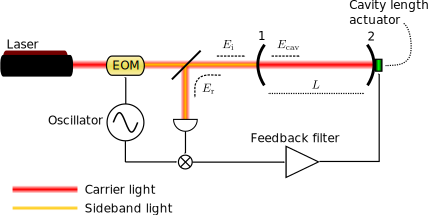
\includegraphics{figs-ifo/resonantcav.pdf}
  \end{center}
  \caption[Diagram of a resonant cavity and control system]{Diagram of a resonant cavity and control system. In this representation, the cavity is held on resonance by feeding back to the position of the end mirror. Alternatively, resonance can be acheived by feeding back to the laser frequency, causing the laser wavelength to follow the length of the cavity.}
  \label{fig:resonantcav}
\end{figure}

We may consider the interference condition after steady state has been acheived as there being a intracavity field, $E_{\rm{cav}}$, which is made up of some of the input light, $E_{\rm i}$ which has been transmitted, and some cavity light which has made a round trip path through the cavity. %NL%
The arrangement of the fields may be seen in Figure \ref{fig:resonantcav}.
\begin{equation}
E_{\rm{cav}}=t_1 E_{\rm i} + r_1 r_2 e^{i 2 k L} E_{\rm{cav}},
\end{equation}
where $r_j$ and $t_j$ are the amplitude reflection and transmission coefficients of the cavity mirrors, for $j=\{1,2\}$ with 1 being the label of the input mirror, and 2 being the label of the end mirror. %NL%
This allows us to solve for the intra-cavity field
\begin{equation}
E_{\rm{cav}}=\frac{t_1}{1 - r_1 r_2 e^{i 2 k L}} E_{\rm i}.
\end{equation}
The reflected field is
\begin{equation}
E_{\rm{r}}=-r_1 E_{\rm i} + t_1r_2 e^{i 2 k L} E_{\rm{cav}}=\frac{-r_1+(r_1^2+t_1^2)e^{i2kL}r_2}{1-r_1r_2e^{i2kL}}E_{\rm i}.
\end{equation}
Assuming no loss of the input mirror ($r_1^2+t_1^2=1$), the cavity field contains a factor of $r_2-r_1$ on resonance. %NL%
Thus the sign of the reflected field on resonance depends on the relative magnitudes of the reflectivities of the cavity mirrors. %NL%
In fact, when the reflectivities are equal, one has perfect impedence mathcing and no field is reflected. %NL%
The case of $r_2>r_1$ is known as overcoupled, and the reflected field changes sign when passing through resonance. %NL%
When $r_2<r_1$, there is no sign change, and this is known as undercoupled. %NL%
The case when no field is reflected ($r_2=r_1$) is known as critically coupled. %NL%
The LIGO arm cavities (Section \ref{sec:armcav}) are an example of strongly overcoupled cavities, while the output mode cleaner (Chapter \ref{ch:omc}) is a critically coupled cavity. %NL%
Undercoupled cavities are more rare because the majority of the light does not penetrate the cavity and thus does not provide a very sensative measurement.

The phase change on reflection is enhanced relative to the phase change inside the cavity. %NL%
For a change of the intracavity phase $\phi = k L$, the phase of the reflected field will change as
\begin{equation}
\phi_r=2\tan^{-1}\left(\frac{2\mathcal{F}}{\pi}\phi\right),
\end{equation}
where $\mathcal{F}$ is known as the \emph{cavity finesse} and has the approximate value $\mathcal{F}\approx \pi\frac{\sqrt{r_1r_2}}{1-r_1r_2}$ where the approximation is valid for $\{r_1,r_2\}\approx 1$. %NL%
For large values of the finesse, the phase of the reflected field has a steep variation compared to the intracavity phase. %NL%
A very typical cavity may have a value of the finesse which is a few hundred. %NL%
Colloquially this can be viewed in the particle picture of light that the photons bounce around in the cavity many times before exiting and thus experience an accumulated phase gain many times that of a single round trip.

%\infobox{Coupling conditoin of a resonant cavity}{
%\begin{wrapfigure}{r}{.4\textwidth}
%\begin{tabular}{|p{5cm}|}
%Coupling condition of a resonant cavity\\
%\begin{itemize}
%\item $r_1<r_2$: Overcoupled, reflected field changes sign on resonance.
%\item $r_1>r_2$: Undercoupled, no sign change on resonance.
%\item $r_1=r_2$: Critically coupled, no field reflected on resonance.
%\end{itemize}
%\end{tabular}
%\end{wrapfigure}
%}
\section{Pound-Drever-Hall reflection locking}
Pound-Drever-Hall (PDH) reflection locking is a powerful technique by which the resonance condition of a laser incident on an optical cavity may be controlled by use of a feedback control system \cite{PDH}. %NL%
In this control system, the error signal is a measurement of the detuning of the laser light from resonance. %NL%
In the case of a fixed length cavity, this may be understood as a measurement of the fluctuations in the laser wavelength. %NL%
We are instead concerned with a very stable laser source and a cavity which may change length due to external influences.\footnote{A gravitational wave changes the phase accumulated in the cavity, which is essentially interchangable with the optical path length of the cavity.} In this case, the error signal is better understood as a measurement of the length changes of the cavity.

As was shown in the previous section, the phase shift of the beam reflected from the resonant cavity is enhanced for fields resonant in the cavity. %NL%
However, for fields not resonant in the cavity, there is nearly no phase shift of the reflected beam. %NL%
The PDH sensing technique exploits this fact by contructing an input beam with frequency components that are both resonant and non-resonant. %NL%
By doing a relative phase measurement of the reflected fields, one may determine length changes of the cavity.

Creation of the input beam is done by sending the beam through an optical modulator. %NL%
This usually comes in the form of an \emph{electro optic modulator} (EOM), which is an optical device that has a electronically variable optical path length. %NL%
Applying a periodic electronic signal, usually at radio frequencies (RF), will induce a periodic phase modulation of the laser beam. %NL%
As will be discussed in Section \ref{sec:freqspace}, the primary result of this phase modulation is to impose new optical fields separated in frequency from the original field by the RF modulation frequency. %NL%
These new fields are usually refered to as \emph{phase modulated sidebands}, the central frequency component is refered to as the \emph{carrier}. %NL%
Figure \ref{fig:resonantcav} shows a typical arrangement of a PDH control system. %NL%
The modulation frequency is chosen such that the sidebands are not resonant in the cavity, and thus do not experience a phase shift when the cavity changes length. %NL%
Comparison of the constant sideband phase with the resonating carrier phase through interferometry yields a very sensitive cavity length measurement. %NL%


Because the modulator is varying the phase of the laser field, ideally there is no associated amplitude modulation. %NL%
Mathematically this is represented by the phase sidebands having an imaginary amplitude when compared to the carrier, they have a 90\degrees{} relative angle in the complex phasor plane. %NL%
The arm-cavities are strongly overcoupled, thus when the carrier is exactly centered on resonance, the reflected field experiences a 180\degrees{} phase shift. %NL%
Thus the phase sidebands are still phase sidebands. %NL%
When the carrier is slightly detuned from resonance, the relative angle between the carrier and sidebands changes and what were once pure phase sidebands now have some amount of amplitude component. %NL%
Thus the power in the reflected beam now experiences a modulation. %NL%
Demodulating the power recorded by a photodetector in reflection will provide the desired length error signal.

\section{The Michelson interferometer}
The pre-stabilized laser and input optics systems provide the LIGO interferometers with an extremely stable light source with which to measure phase pertubations. %NL%
To provide a phase sensitivity necessary to detect gravitational waves it will be necessary to play a few tricks to hide our gravitational wave readout system from the noise still present on the input laser.

\begin{figure}
  \begin{center}
  \leavevmode
  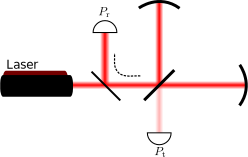
\includegraphics{figs-ifo/michelson.pdf}
  \end{center}
  \caption[Diagram of a Michelson interferometer.]{Diagram of Michelson interferometer. Photodetectors are arranged to measure the transmitted power, $P_{\rm t}$, and the reflected power, $P_{\rm t}$. The interferometer is operated near a dark fringe on transmission, and most of the light is directed to the reflection photodetector.}
  \label{fig:michelson}
\end{figure}

A Michelson interferometer (shown in Figure \ref{fig:michelson}) is composed of a beamsplitter, which usually has a power reflectivity of 50\perc{}, and two highly reflecting mirrors in each arm. %NL%
The laser field propagates down each arm, before reflecting back towards the beamsplitter. %NL%
The two beams then interfere at the beamsplitter and the intensity of light at the reflection and transmission ports vary with the differential length change of the arms. %NL%
The power measured exiting each port is:
\begin{align}
\frac{P_{\rm{t}}}{P_{\rm{BS}}} &= \left(\frac{r_1+r_2}{2}\right)^2\sin^2(kl_-)+\left(\frac{r_1-r_2}{2}\right)^2\cos^2(kl_-),\\
\frac{P_{\rm{r}}}{P_{\rm{BS}}} &= \left(\frac{r_1+r_2}{2}\right)^2\cos^2(kl_-)+\left(\frac{r_1-r_2}{2}\right)^2\sin^2(kl_-),
\end{align}
where $r_{1,2}$ are the amplitude reflectivities of the mirrors, $k=2\pi/\lambda$ is the wavenumber of the light, $P_{\rm{BS}}$ is the power incident on the beamsplitter, and $l_-$ is the difference of the lengths of the rwo arms. %NL%
Thus one may measure the power dependence at one or both ports to measure differential length changes. %NL%
The power dependence at the transmission port is periodic with differential length changes of the interferometer. %NL%
At first glance it might be desirable to make the ``set point'' %NL%
of the interferometer be the place where the power varies most as a function of the differential length. %NL%
In this case, halfway between the maximum and minimum of the fringe would have the greatest derivative and thus would maximize the signal measured for any given length change. %NL%
This ignores, however the dependence of sensing noise on the interferometer set point. %NL%
Shot noise is a fundamental source of measurement uncertainty due to the random arrival of photons on the photodetector. %NL%
For a measurement of the transmitted power $P_{\rm t}$, and assuming $r_1=r_2=1$, the amplitude spectral density of the shot noise is:
\begin{equation}
\label{eqn:michshotnoise}
N_{\rm{shot}}=\sqrt{2\frac{hc}{\lambda}P_{\rm i}\sin^2(kl_-)}.
\end{equation}
For a static interferoemeter set point $l_-$ with a small length variation $\delta l$, the resulting signal will be
\begin{equation}
S=\frac{\partial P_{\rm i}}{\partial l_-}(l_-) \times \delta l = 2P_{\rm i}\sin{(kl_-)}\cos{(kl_-)}\times k\delta l
\end{equation}
We may then determine the signal to noise ratio (SNR) of measurements of the differential length change of the interferometer. %NL%
The noise varies as $|\sin(kl_-)|$ while the signal varies as $\sin(kl_-)\cos(kl_-)$, thus the SNR will vary as $\cos(kl_-)$. %NL%
As one can see, the maximum of the magnitude of the signal to noise is acheived at $kl_- = m \lambda$ for $m \in \mathbb{Z}$, which is (quite counter intuitively!) when no light is on the photodetector. %NL%
In practice, some small amount of light will need to be on the photodetector so that the signal can overcome other sources of sensing noise. %NL%
Though, as long as the offset remains small, the SNR approaches the maximum value. %NL%
Applying this scheme of using a small static offset of the Michelson fringe to the initial LIGO detectors was one of the major upgrades performed in Enhanced LIGO. %NL%
Other benefits of using this technique over a RF demodulation style technique is discussed in Section \ref{sec:dcreadout}.

Using the analogy which treats the laser wavelength as a ruler with which one measures optical path length, there is an intuitive picture which shows why the correct arrangement of a Michelson interferometer may be made insensitive to fluctuations of your ruler. %NL%
Because the beamsplitter directs the same laser source to each arm, it is obvious that fluctuations of the laser wavelength (our ruler) will be identical in both arms. %NL%
This is a problem if one desires to measure the average length of the two arms, fluctuations in your ruler will directly cause fluctuations in your measurement. %NL%
If, instead, the differential arm length change is the desired measurement, ruler length fluctuations are supressed. %NL%
For these reasons, both amplitude and phase fluctuations of the laser light are common mode and thus supressed when making a differential measurement of the arm lengths. %NL%
This is covered quantitatively in Section 10.4 of Malik Rakhmanov's thesis \cite{Rakhmanov}.

To maximize the differential arm phase difference of a gravitational wave, one should choose the angle between the Michelson arms to match the ``shape'' %NL%
of the waves. %NL%
As seen in Chapter \ref{ch:gws}, gravitational waves stretch and squish along perpendicular axes. %NL%
Therefore the most common arrangement of a michelson (90\degrees{}) also happens to be the optimum for detecting gravitational waves.

\section{Michelson with arm-cavities}
\label{sec:armcav}
One may exploit the common mode rejection of laser noise provided by the Michelson interferometer, while taking advantage of the high phase sensitivity of a resonant cavity, by joining the two designs. %NL%
The LIGO detectors acheive this by converting both arms of the Michelson each into resonant cavities. %NL%
This is heuristically similar to making a Michelson with much longer arms due to the phase gain of the arm cavities.

The resonance condition enforced by the control systems is that a half-odd integer number of wavelengths fit in the length of the cavity, or $L=n\lambda/2$ for some large integer $n$. %NL%
In terms of the optical frequency $f$ this is $L=nc/f$. %NL%
Thus if the control system holds the cavity on resonance by modifying the laser frequency, $\delta f$, and there is a length change $\delta L$,
\begin{align}
\delta L &= -\frac{nc}{f^2}\delta f,\notag \\
\frac{\delta L}{L} &= -\frac{\delta f}{f}.
\label{eqn:dfdL}
\end{align}
Thus one may stabilize the frequency noise of a laser by locking the laser to some cavity. %NL%
Provided that the length of the cavity is sufficiently stable, this may be used to reduce the frequency noise of the laser below its intrinsic level. %NL%
Additionally, according to Equation \ref{eqn:dfdL}, this becomes more effective as the cavity is made longer.

This shows a trick one may play once the effort has been spent to build two arm-cavities. %NL%
We saw above that the common arm length of the interferometer may be difficult to measure due to laser frequency noise. %NL%
So it is not pracical to use the common arm mode as a gravitational wave sensor. %NL%
To not let effectivly half of one's interferometer go to waste, one may exploit this additional opical cavity as a stable length reference. %NL%
This is known as the \emph{common mode servo}.

\section{Power recycling}
Apart from the small fraction of light which is lost due to absorption or scattering, most of the light incident on a michelson interferometer operating on the dark fringe is reflected back from the input port toward the laser. %NL%
The solution to this very un-green situation is that the light can be directed back into the interferometer using a technique known as \emph{power recycling}. %NL%
The most straightforward way to understand power recycling is to consider the interferometer as a kind of mirror. %NL%
If one places another mirror, called the power recycling mirror (PRM), between the laser and interferometer, the new system forms a resonant cavity. %NL%
A careful choice of the reflectivity of the power recycling mirror makes this resonant cavity critically coupled, and thus a minimal amount of light is reflected back toward the laser. %NL%
In the case of LIGO, the power incident on the beam splitter can be enhanced by a factor of around 50, which correspondingly decreases the shot noise as in Equation \ref{eqn:michshotnoise}. %NL%


\section{Sensing and control of a power recycled Michelson interferometer with arm-cavities}
\begin{figure}
  \begin{center}
  \leavevmode
  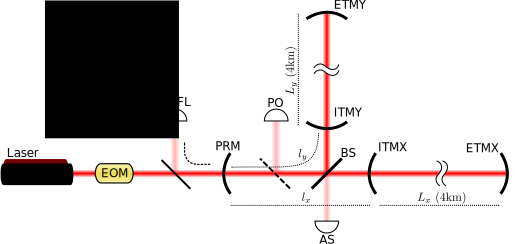
\includegraphics{figs-ifo/prfpmi.pdf}
  \end{center}
  \caption[Diagram of a power-recycled Fabry-Perot Michelson interferometer.]{Diagram of a power-recycled Fabry-Perot Michelson interferometer. This is a simplified version of the optical configuration of the LIGO interferometer. Also shown are the definitions of the canonical length degrees of freedom.}
  \label{fig:prfpmi}
\end{figure}
The optical setup of the full LIGO interferometer is quite a bit more complicated than that of a single cavity. %NL%
To maintain the resonance condition of the entire interferometer, it is necessary to sense and control four independent length degrees of freedom. %NL%
It so happens that the technique of PDH reflection locking is well adapted for sensing the length degrees of freedom of more complicated interferometers. %NL%
Placing one's photodetectors at the correct ports of the interferometer can provide all needed information for length sensing. %NL%
The canonical reference on the topic is \citet{Fritschel:01}, but we will provide a short summary.

As seen in Figure \ref{fig:prfpmi}, the interferometer is composed of six primary mirrors. %NL%
Theses are the \emph{power recycling mirror} (PRM), the \emph{beamsplitter} (BS) and the arm cavity optics, refered to as the \emph{end test mass} (ETM) and \emph{input test mass} (ITM), one for each arm, labeled X and Y. %NL%
Only four degrees of freedom are relevent and measurable by their optical path length. %NL%
In the case of LIGO, the degrees of freedom of all the mirrors are measured relative to the ITMs. %NL%
The basis chosen to represent theses lengths is shown in Figure \ref{fig:prfpmi}. %NL%
The length degrees of freedom are refered to as the \emph{differential arm length} (DARM), the \emph{common arm length} (CARM), the \emph{power recycling cavity length} (PRC) and the \emph{Michelson length} (MICH).

Due to the optical topology and location of the sensors, the different sensing ports provide information about the various degrees of freedom of the interferometer. %NL%
As in PDH, the light is phase modulated at RF frequencies before being injected into the interferometer and the length signal is encoded as an RF amplitude modulation of the photodetector power. %NL%
Photodetectors are located at several output ports of the interferometer. %NL%
The modulation can be in the cosine (in-phase, I) or sine (quadrature-phase, Q) quadratures. %NL%
The length degree of freedom with most sensitivity to gravitational waves is DARM, which is the primary signal present at the antisymmetric (AS) port, though the AS port also has some contribution from MICH. %NL%
MICH is the dominant contribution to the power recycling cavity pickoff (PO) port in the Q phase. %NL%
The I phase of the PO port, and the reflection (REFL) port, both have a primary contribution from CARM, with a small contribution from PRC. %NL%
This presents the difficult task of having two sensors which are nearly degenerate in the sensed degree of freedom. %NL%
In LIGO this is solved due to the very high gain of the common mode servo. %NL%
The common mode servo strongly supresses the REFL signal, creating a gain hierarchy with the PO-I signal. %NL%
The signal which remains in PO-I is purely PRC.

The next generation of interferometers, including Advanced LIGO, will include an additional signal recycling mirror which sits between the BS and the AS port. %NL%
This adds an additional length degree of freedom which further complicates the sensing and control \cite{T1000298}.

\section{Non-modulated (DC) readout}
\label{sec:dcreadout}
Prior to the beginning of Advanced LIGO, there was a incremental upgrade called Enhanced LIGO. %NL%
One of the modifications performed during the Enhanced LIGO upgrade was to change the scheme for sensing the DARM degree of freedom. %NL%
The DC power at the AS port has a quadratic dependance on DARM. %NL%
Thus if the arm cavities are differentially detuned slightly (on the order of 10 picometers) from resonance, there will be a linear dependence of the DC power from DARM. %NL%
An alternate picture of the scheme is that in the RF scheme, the RF sidebands are the local oscillator which beats against the gravitational wave sidebands to produce an RF signal, which is a form of heterodyne detection. %NL%
While in the DC case, the DARM offset produces a local oscillator at the same baseband frequency as the signal sidebands, which is a form of homodyne readout. %NL%
A photodetector which measures this DC power is an alternative sensor for reading out DARM. %NL%
DC readout of DARM has been implemented on the GEO600 detector \cite{GEODC}, the Caltech 40 meter prototype interferometer \cite{40mDC}, and for Enhanced LIGO \cite{Tobin}. %NL%
DC readout of DARM is also part of the baseline design for Advanced LIGO. %NL%
A very thorough treatment of the subject can be found in Tobin Fricke's PhD dissertation \cite{FrickeThesis}. %NL%
Here we will cover some of the benefits of such a scheme.

Light which resonates in the compound system composed of the arm cavities and the power recycling cavity experiences an effective cavity bandwidth which is much more narrow than the bandwidth of the arm cavities alone \cite{Rakhmanov}. %NL%
This narrow bandwidth acts as a effective low pass filter of the laser noise fluctuations on the light. %NL%
In the LIGO interferometers, the carrier light is resonant in the coupled cavity system and experiences a filter with a corner frequency of approximately 1Hz. %NL%
The RF sidebands do not resonate in the arm cavities and thus do not experience such dramatic filtering. %NL%
The carrier light thus serves as a much quieter local oscillator than the RF sidebands. %NL%
Thus switching to DC readout can reduce many laser noise couplings.

There is an intrinsic reduction in the shot noise when going from RF to DC readout. %NL%
The total power on the detector is modulated at twice the frequency of the RF sidebands due to the beating of the upper and lower sidebands with eachother. %NL%
The RF demodulation of DARM preferentially samples the signal at the peaks of the RF modulation, leading to a shot noise contribution higher than the DC case by a factor of $\sqrt{3/2}$. %NL%
There is a very nice treatment of this effect in Section 2.9 of Tobin Fricke's dissertation \cite{FrickeThesis}.

One of the drawbacks of DC readout is that the audio modulation of any of the optical fields present at the AS port can cause noise in the readout. %NL%
To mitigate the existence of the fields not necessary for producing the signal, i.e. %NL%
any fields that are not the local oscillator or the signal fields, one may utilize an output mode cleaner. %NL%
The output mode cleaner acts as both a spatial and frequency filter of the fields detected at the AS port and will be described in detail in the following chapter.

\chapter{The output mode cleaner}
\label{ch:omc}
One of the primary components of the Enhanced LIGO upgrade was the addition of an output mode cleaner or OMC \cite{T060156}. %NL%
This chapter describes the motivation for installing and OMC and some measurements of the performance of the OMC installed on the H1 interferometer at the LIGO Hanford Observatory.

\section{Motivation for an OMC}
The interferometer is supplied with a beam that has a very nearly pure Gaussian spatial profile thanks to the input mode cleaner. %NL%
The input mode cleaner is a nearly critically coupled resonant optical cavity which filters the beam supplied by the laser before it is delivered to the interferometer input. %NL%
The power recycling cavity builds up power and delivers it to the long arms. %NL%
The arms further recycle the laser light and this large resonant field acts as the source field that gets modulated by a passing gravitational wave and pumps light into sidebands at the gravitational wave frequency. %NL%
The gravitational wave signal on the PD comprises the beat note of these audio frequency sidebands with a strong coherent field. %NL%
Although the beam delivered by the input mode cleaner is spatially very pure, the efficiency of coupling this beam to the final resonant mode of the arm cavity is not ideal. %NL%
Components of the input light that are not matched to the mode of the arm cavity will not resonate and some of this unmatched light will exit the antisymmetric port along with the signal light. %NL%
The unmatched light at the antisymmetric port will exist as higher order modes (HOM) relative to the arm cavity mode and is often referred to as ``junk light.'' %NL%
The presence of this light on a photodetector will contribute photon shot noise. %NL%
Also, if the coupling is time dependent, the time variation of the junk light directly contaminate the signal with noise.

It is, therefore, desirable to be able to separate the junk light from the signal rich audio frequency fields originating in the arm cavities. %NL%
A critically coupled resonant optical cavity is a natural spatial filter for light. %NL%
When placed at the output of the interferometer between the AS port and the PD, as seen in Figure \ref{fig:omclocation}, we refer to such a cavity as the output mode cleaner (OMC).

\begin{figure}
  \begin{center}
  \leavevmode
  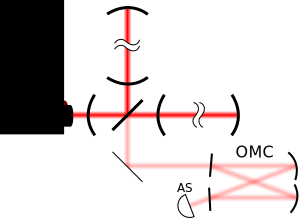
\includegraphics{figs-omc/omclocation.pdf}
  \end{center}
  \caption[Diagram showing the location of the OMC.]{Diagram showing the location of the OMC. This diagram is not drawn to scale.}
  \label{fig:omclocation}
\end{figure}

It can be useful to point out that interferometers based on both RF and DC readout can benefit from an OMC. %NL%
Both the GEO and Virgo interferometers have used OMCs in an RF readout configuration, and LIGO experimented with an OMC before using DC readout \cite{G040326}. %NL%
An OMC is especially important for a DC readout interferometer because any audio frequency modulation of fields that are not the local oscillator or signal will contaminate the readout. %NL%
Because readout is performed at DC, all audio frequency interference of the fields will directly couple to the signal channel, as opposed to an RF heterodyne scheme where the signal is shifted away from low frequency interference. %NL%
An OMC may also be used to ensure that the light provided by the differential arm offset dominates the DC power present on the detection photodiode, otherwise DC power from other fields (such as the RF sidebands) will contribute to photon shot noise without increasing the signal strength. %NL%


Thus, for an interferometer that employs DC readout, the OMC should efficiently strip the HOM field components of the carrier field as well as the RF sidebands. %NL%
This is achieved by creating a cavity with a narrow linewidth, capable of transmitting the desired (carrier) field, while filtering out higher frequencies. %NL%
Ideally, being a critically coupled optical cavity, light incident on the OMC is totally transmitted on resonance. %NL%
The normalized transmission of the off-resonant fields is given by
\begin{equation}
\label{eqn:finesse}
\frac{T}{T_0}=\frac{1}{1+\frac{4}{\pi^2}\mathcal{F}^2\sin{}^2\phi},
\end{equation}
where $\mathcal{F}$ is known as the \emph{cavity finesse} (see also Section \ref{sec:finesse}) and $\phi$ is the detuning from resonance. %NL%
In terms of a frequency detuning of $\Delta f$ of the incident light, $\phi = \pi \Delta f / \mathrm{FSR}$. %NL%
The FSR is the frequency spacing of successive resonances, discussed in Section \ref{sec:FSR}.

\section{Optical and mechanical design of the OMC}
\begin{figure}
  \begin{center}
  \leavevmode
  \includegraphics{figs-omc/omcphoto.pdf}
  \end{center}
  \caption[Photograph of the OMC.]{Photograph of the OMC. The strong red line shows the primary beam path. The light red line shows the QPD sample of the input beam. Only shown are the QPD and transmission PD tombstones, the actual photodetectors are not mounted in this photograph. Photograph credit to Sam Waldman.}
  \label{fig:omcphoto}
\end{figure}
Prior to Enhanced LIGO, experiments were performed using a OMC borrowed from the GEO600 interferometer to investigate the difficulties in using an OMC with LIGO. %NL%
Noise introduced from jitter of the OMC input beam due to air currents and mechanical vibrations spoiled the sensitivity of the LIGO detector when the OMC was used. %NL%
Consequently, one of the most obvious lessons learned from these investigations was the need to house the OMC in a low vibration environment. %NL%
For Enhanced LIGO, it was decided that the OMC would be housed inside the vacuum system and would be isolated from vibrations of the environment through the use of a seismically isolated optics table as well as a suspension system to provide passive filtering of vibrations.

\subsection{Cavity optics}
The design of the OMC was chosen to be a four mirror bow-tie cavity. %NL%
This choice was made over that of a two mirror linear cavity so that there was spatial separation of the reflected beam. %NL%
An even number of mirrors was chosen such that the horizontal and vertical HOMs would experience the same overall phase shift and thus experience nearly the same frequency offset from resonance, reducing the chances of an accidental HOM resonance.

\begin{figure}
  \begin{center}
  \leavevmode
  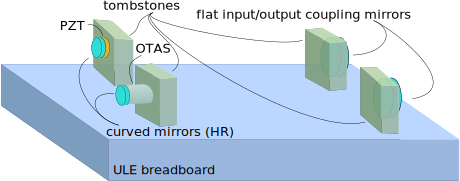
\includegraphics{figs-omc/construction.pdf}
  \end{center}
  \caption[Diagram of OMC cavity components]{Diagram of OMC cavity components. Auxiliary optics and sensors are not shown. The tombstones have holes (not pictured) machined in them to allow the laser beam to pass through (see Figure \ref{fig:inputcouplerphoto} for a photograph of the input coupler and tombstone.)}
  \label{fig:omcconstruction}
\end{figure}

\begin{figure}
  \begin{center}
  \leavevmode
  \includegraphics{figs-omc/inputcouplerphoto.pdf}
  \end{center}
  \caption[Close up photograph of the OMC input coupler mirror.]{Close up photograph of the OMC input coupler mirror. The photograph is taken from the in-cavity side of the optic.}
  \label{fig:inputcouplerphoto}
\end{figure}

A diagram of the OMC may be seen in Figure \ref{fig:omcconstruction}. %NL%
The OMC optics are bonded with Vacseal epoxy onto custom designed fused silica optics mounts, called tombstones. %NL%
 The tombstones were then bonded to a slab of Corning ultra-low expansion (ULE) Glass\footnote{The dimensions of the OMC breadboard are 450mm$\times$150mm$\times$39mm} with UV cure epoxy from Optocast, which we will refer to as the \emph{OMC breadboard}, pictured in Figure \ref{fig:omcphoto}. %NL%
Figure \ref{fig:inputcouplerphoto} shows the OMC input coupler mirror and tombstone, bonded to the breadboard. %NL%
This arrangement fixed the cavity length to the desired value and was designed to be stable against thermal variation. %NL%
The microscopic cavity length was controlled using a pair of actuators. %NL%
A fast PZT between one of the optics and its tombstone acted as a low range (1/10 of a wavelength) high bandwidth (5kHz) length actuator. %NL%
Long range (several wavelengths) actuation was provided by one cavity mirror situated at the end of an aluminum tube heated by a ceramic heating element, affectionately referred to as the OTAS.\footnote{OMC Thermal Actuation System}

A mode cleaner cavity is purposefully designed such that HOMs do not occupy a degenerate resonance with the resonant \TEM{00} mode (see Section \ref{sec:modecleanap} on how a mode cleaner acts as a filter of transverse modes). %NL%
Cavities are commonly characterized by their stability $g$-parameter.\footnote{Asymmetric cavities are often given two $g$-parameters, one for each mirror (labeled 1 and 2) and $g=\sqrt{g_1 g_2}$.} The Gouy phase shift, $\eta$, is the phase shift of a focused \TEM{00} beam relative to a plane electromagnetic wave. %NL%
The round trip Gouy shift in the cavity is determined by the cavity geometry as
\begin{equation}
\label{eqn:gouyg}
\cos(\eta)=g,
\end{equation}
where the $g$-parameter is usually given by $g=1-L/R$ for a linear cavity of length $L$ and mirror radius of curvature $R$ \cite{T080208}. %NL%
The OMC is not a linear cavity, the light travels the length of the cavity only once during a full round trip. %NL%
To avoid confusion we will use the \emph{perimeter}, $p$, to denote the full round trip length. %NL%
One may substitute $2L=p$ in most formulae for linear cavities. %NL%
An extensive analysis was done by Sam Waldman to determine the optimal cavity geometry to minimize the transmission of off-resonant HOM and frequency components through the OMC \cite{T080144}. %NL%
The final design of the OMC was chosen to have a perimeter length of 1.042m, with 2m radius of curvature curved optics, giving a $g$-parameter of 0.7395 and a Gouy phase shift of $0.235\pi$ radians. %NL%
This implies that the fourth-order HOMs will accumulate almost $\pi$ radians relative to the \TEM{00} mode and be somewhat close to resonance.

\subsection{Sensors and auxiliary optics}

The gravitational wave signal readout is derived from the OMC transmitted power. %NL%
The light transmitted by the OMC is split by a near 50/50 beam splitter and detected on two photodiodes. %NL%
Both the beam splitter and photodiodes are located on the OMC breadboard. %NL%
The beamsplitter is glued to a tombstone similar to that of the cavity optics. %NL%
The photodiodes were attached to tombstones via a sandwich of metal plates screwed together around the tombstone. %NL%
This arrangement ensured that the OMC transmitted beam would not drift relative to the readout detectors.

A steering mirror on the OMC breadboard transmitted a small sample of the incoming beam allowing the input pointing to be analyzed by two quadrant photodetectors (QPDs). %NL%
A 50/50 beam splitter distributed equal amounts of the input beam to the two QPDs. %NL%
The QPDs were located at different distances from the beam splitter to allow both beam angle and lateral position to be measured. %NL%
The location of all the OMC sensors can be seen in Figure \ref{fig:omcphoto}.

\subsection{Suspension system}
\begin{figure}
  \begin{center}
  \leavevmode
  \includegraphics{figs-omc/susphoto.pdf}
  \end{center}
  \caption[Photograph of the OMC double pendulum suspension.]{Photograph of the OMC double pendulum suspension. The line sketch shows the upper mass stage, which is obscured in the photograph by the coil actuators.}
  \label{fig:susphoto}
\end{figure}

The OMC breadboard was suspended from a two stage vibration isolation suspension, pictured in Figure \ref{fig:susphoto}. %NL%
On the optics table was a large steel frame which housed the OMC. %NL%
An upper mass stage was suspended from the frame by two pendulum wires attached to the ends of blade springs. %NL%
The OMC breadboard was then suspended by four more wires attached to blade springs from the upper mass stage. %NL%
Servo control provided feedback damping of the suspension eigenmodes. %NL%
All actuation and sensing was performed on the intermediate stage, with actuation provided by electromagnetic coil actuators attached to the cage which applied forces to permanent magnets attached to the upper mass. %NL%
The actuator module also housed the sensing system which consisted of LED shadow sensors which measured the position of protruding flags attached to the magnets used for actuation.

\subsection{Mode matching telescope}
\begin{figure}
  \begin{center}
  \leavevmode
  \includegraphics{figs-omc/ttphoto.pdf}
  \end{center}
  \caption[Photograph of a Tip Tilt optic.]{Photograph of a Tip Tilt optic. The original Tip Tilt design is shown, before being retrofitted with blade springs. Alignment actuation control is provided by coil actuators coupled to permanent magnets housed in the mirror holder. }
  \label{fig:ttphoto}
\end{figure}
The beam exiting the interferometer from the antisymmetric port was directed through a beam steering and mode matching telescope. %NL%
The purpose of such a telescope is to correctly align and focus the beam exiting the interferometer to maximize the transmission of the gravitational wave signal through the OMC.

The steering optics were housed in a single pendulum suspension system. %NL%
The suspension and optics were collectively referred to as \emph{Tip-Tilt optics},\footnote{The Tip Tilts were designed by B. %NL%
Slagmolen of the Australian National University\cite{T0900096}.} one of which is pictured in Figure \ref{fig:ttphoto}. %NL%
The mounting and suspension of the beam steering optics underwent several modifications during the Enhanced LIGO project (see Chapter \ref{ch:jitter}). %NL%
The final configuration consisted of three highly reflective curved mirrors. %NL%
Two suspended by a single pendulum stage, with vertical isolation provided by blade springs, and a coil-magnet/shadow sensor system similar to that used in the OMC suspension. %NL%
The actuator system allowed feedback control of the optic angle for active beam alignment. %NL%
The third was housed in a similar suspension system, but without any sensing or actuation capabilities.

\subsection{Vibration isolation table}
The Tip-Tilts and OMC suspension frame were all housed in a single vacuum chamber and situated on top of a actively controlled seismic isolation table, the HAM-ISI.\footnote{HAM chamber Internal Seismic Isolation system} The HAM-ISI employed a single stage of passive vibration isolation, coupled with active feedback control using inertial sensors as the primary error signal. %NL%
A thorough account of the HAM-ISI design and performance is given in Chapter 5 of Jeff Kissel's thesis \cite{kisselthesis}.

\section{Characterization of the H1 OMC}
\begin{figure}
  \begin{center}
  \leavevmode
  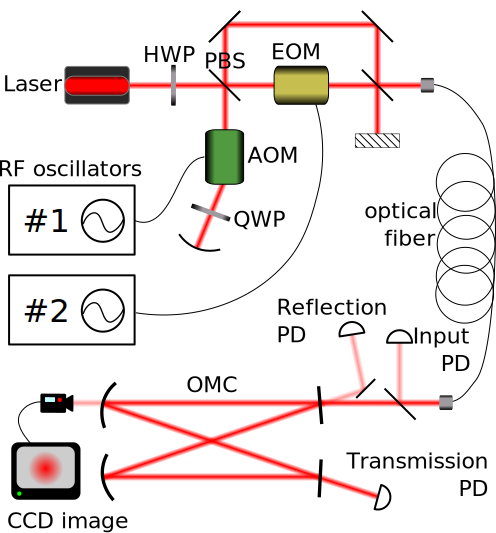
\includegraphics{figs-omc/interrogator.pdf}
  \end{center}
  \caption[Block diagram of OMC characterization setup.]{Block diagram of OMC characterization setup, also known as the OMC interrogator. The setup provides single mode laser light with RF sidebands for reflection locking, as well as a subcarrier with a tunable frequency.}
  \label{fig:interrogator}
\end{figure}

Figure \ref{fig:interrogator} shows a diagram of the experimental setup used to measure several parameters of the OMC that was installed on the H1 LIGO interferometer in Hanford, WA. %NL%
These measurements were done prior to the installation of the OMC into the interferometer. %NL%
The laser source is a Nd:YAG NPRO providing a 1064nm wavelength laser beam. %NL%
The polarization is rotated by a half-wave plate (HWP). %NL%
A polarizing beam splitter (PBS) sends some fraction of the light through an electro-optic modulator (EOM) which is driven at by RF oscillator \#2. %NL%
The fraction transmitted by the PBS is tuned by changing the angle of the HWP. %NL%
The EOM introduces two RF sidebands which will be used for cavity length control. %NL%
The other path of light is directed to an acousto-optic modulator (AOM). %NL%
The light is double passed though the AOM and and receives a frequency shift which is twice the frequency of RF oscillator \#1. %NL%
A quarter-wave plate (QWP) causes the polarization to rotate 90\degrees{} after double passing, causing both paths to now be in the same polarization. %NL%
The light from the two paths are recombined before being injected into an optical fiber. %NL%
The frequency makeup of the combined beam includes the original carrier frequency, two RF sidebands and a frequency shifted subcarrier.

The light exiting the other end of the optical fiber is incident on the input coupling mirror of the OMC cavity. %NL%
A small sample of the input beam is incident on a photodetector. %NL%
The promptly reflected beam is detected on a photodetector where the photocurrent is demodulated at the frequency of RF oscillator \#2 for a PDH style locking scheme. %NL%
The frequency of oscillator \#2 is chosen so that it is outside of the OMC resonance when the carrier is in resonance. %NL%
This provides an error signal which is fed back to the frequency actuator of the laser. %NL%
The control system is able to maintain resonance of the laser in the OMC. %NL%
The laser transmitted through the OMC is detected on another photodetector. %NL%
A very small sample of the light in the cavity is transmitted through one of the HR mirrors and detected by a CCD sensor.

\subsection{Free spectral range}
\label{sec:FSR}
Resonance occurs in the cavity when the total round trip phase of the incident laser beam as it propagates through the cavity is an integer multiple of $2\pi$. %NL%
In terms of the frequency of the laser beam, this occurs at multiples of what is called the \emph{free spectral range} (FSR). %NL%
The FSR is related to the round trip cavity perimeter $p$ by $\mathrm{FSR}=c/p$.

The technique used to measure the cavity FSR involved locking the laser frequency so the carrier was resonant in the OMC while varying the frequency of the subcarrier, causing it to pass through resonance, and measuring the OMC transmitted power. %NL%
The OMC transmitted power will be maximized when the subcarrier is separated from the carrier by a multiple of the FSR.

The RF frequency generator was tuned to maximize the subcarrier transmission. %NL%
The error was estimated to be the smallest frequency step that did not cause a noticeable change in transmission. %NL%
The measured FSR is
\begin{equation}
\mathrm{FSR}=278.288\pm0.001\text{MHz}.
\end{equation}
This corresponds to a cavity perimeter of 1.077m. %NL%
The length differs from the design value, though the purpose of the design was that the fourth order modes are close to, but outside of resonance, as measured in the following section.

\subsection{Higher order mode spacing}
Similarly, the higher order mode frequency shift is measured by varying the subcarrier frequency until the subcarrier is resonant on a higher order mode of the OMC \cite{Uehara:95}. %NL%
Coupling of the subcarrier beam into the HOMs is enhanced if slight misalignments are introduced on the input beam. %NL%
The identity of the higher order mode is determined by the image recorded by the CCD camera.

The HOM field components experience an effective frequency shift relative to the \TEM{00} carrier field due to the Gouy phase shift. %NL%
The effective frequency shift is given by
\begin{equation}
\label{eqn:gouyshift}
(m+n)\eta=\pi\frac{\Delta f}{\mathrm{FSR}}\mod \pi
\end{equation}
where $m$ and $n$ are the \TEM{mn} mode indices, $\Delta f$ is the frequency shift, and $\eta$ is the Gouy phase shift, which is related to the cavity $g$-parameter by Equation \ref{eqn:gouyg}. %NL%


\begin{table}
  \begin{center}
    \begin{tabular}{lll|ll}
      \hline
      $m$ & $n$ & $\Delta f$ & $\eta$ & $g$ \\
      \hline
      0 & 1 & -489.60 MHz & 0.2407$\pi$ & 0.7275\\
      1 & 0 & -489.12 MHz & 0.2424$\pi$ & 0.7238\\
      0 & 4 &  267.96 MHz & 0.2407$\pi$ & 0.7274\\
      4 & 0 &  269.60 MHz & 0.2422$\pi$ & 0.7242\\
      \hline
    \end{tabular}
  \caption[Higher order mode frequency shifts in the OMC]{Higher order mode frequency shifts in the OMC. The frequency shift measured by varying the subcarrier separation from the resonating carrier. The $m$ index is the horizontal mode order. Negative frequency shifts were achieved by using the -1 diffraction order of the AOM.}
  \label{tab:HOM}
  \end{center}
\end{table}

Table \ref{tab:HOM} shows the measurements for several higher order mode frequency shifts. %NL%
Notice that the horizontal and vertical modes experience slightly different Gouy shifts in the cavity. %NL%
This is due to the astigmatism introduced in the cavity by non-normal incidence on the cavity mirrors. %NL%
One may use the measured $g$-parameters to estimate the radius of curvature of the curved optics of the OMC. %NL%
If we take the average value of the measured $g$-parameter, this implies a radius of curvature of 1.96m, which is close to the specification of 2m.

These data were taken with the OMC at room temperature. %NL%
It was later discovered that the HOM spacing varied with the temperature of the thermal length actuator \cite{OTASmodes}\footnote{Note that all ilog references may be viewed publically with username {\it reader} and password {\it readonly}.}. %NL%
With high enough temperature, this would bring the fourth order modes in coincidence resonance with the \TEM{00} mode! %NL%
We postulated that this was due to a change in the effective radius of curvature of the OTAS mirror as the OTAS expanded. %NL%
To mitigate this, the temperature was kept low during operation.

\subsection{Cavity finesse}
\label{sec:finesse}
The frequency profile of the transmitted peak when the subcarrier is shifted through resonance may be used to determine the cavity finesse. %NL%
The finesse is defined as the ratio of the spacing between resonances (the FSR) to the full width at half maximum (FWHM) of the resonance. %NL%
In the experiment, a sawtooth wave was used to sweep the subcarrier offset frequency while the OMC transmission was monitored. %NL%
These signals were digitized and recorded. %NL%
The recorded transmission versus frequency shift data are shown in Figure \ref{fig:finesseFit}. %NL%
The curve fit model used was Equation \ref{eqn:finesse} with $\phi=\pi \Delta f/\mathrm{FSR}$ and an arbitrary scaling and offset. %NL%
The fitting parameters return a cavity finesse of $367\pm2$.


\begin{figure}[h!]
  \begin{center}
  \leavevmode
  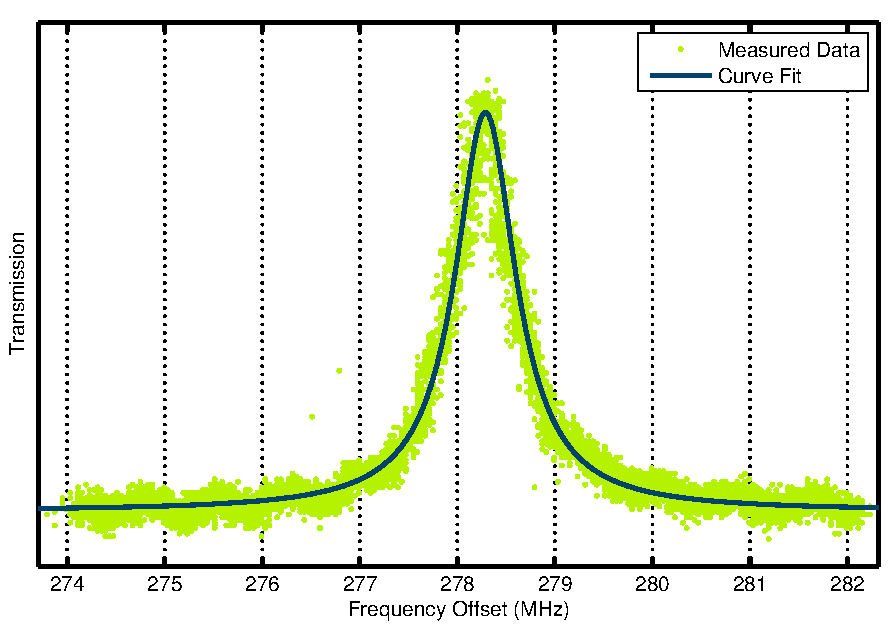
\includegraphics{figs-omc/finesseFit.pdf}
  \end{center}
  \caption[Measurement of the OMC transmission profile.]{Measurement of the OMC transmission profile. The OMC is locked on the carrier, pictured is the transmission while varying frequency offset as the subcarrier passes through resonance. The width of the transmission peak is used to determine the cavity finesse. Fitted parameters give a finesse of $367\pm2$.}
  \label{fig:finesseFit}
\end{figure}

\subsection{Cavity losses}
\label{sec:omclosses}
The intra-cavity loss of the OMC was inferred by using three photodetectors; one measuring a sample of the input light, one measuring the reflected light, and one measuring the transmitted light, as seen in Figure \ref{fig:interrogator}. %NL%
Both the reflection and transmission photodiodes were calibrated relative to the input diode. %NL%
The calibration of the reflection diode was achieved by leaving the input and reflection diodes in place and blocking the beam inside the cavity. %NL%
The relative power readings of the diodes were then recorded and the ratio gives the reflection calibration. %NL%
One must also take into account the known transmission of the OMC input coupling mirror. %NL%
This calibration is done without moving the beam to be used during the measurement and mitigates systematic errors due to variations in the sensitivity over the surface of the diodes. %NL%
The transmission diode, however needed to be moved during calibration to measure the power incident on the cavity. %NL%
The transmission diode was also calibrated relative to the input diode.

This technique measures the light incident on the cavity, reflected from the cavity, and transmitted by the cavity. %NL%
Any incident light which is neither reflected nor transmitted is assumed to be absorbed and constitutes cavity losses. %NL%
Table \ref{tab:lossmeas} shows the data taken to determine the cavity losses. %NL%
The transmission efficiency is defined to be $P_{\text{transmission}}/(P_{\text{input}}-P_{\text{reflection}})$. %NL%
The cavity transmission efficiency was measured to be approximately 96\perc{}.

\begin{table}
  \begin{center}
    \begin{tabular}{lll|l}
      \hline
      Input (V) & Reflection (V) & Transmission (V) & Transmission Efficiency \\
      \hline
      0.95 & 1.51 & 0.53 & 0.965 \\
      0.903 & 1.44 &0.498 & 0.958\\
      \hline
    \end{tabular}
  \caption[Measurements of the OMC intra-cavity losses.]{Measurements of the OMC intra-cavity losses. All units are calibrated in Volts measured by the input PD.}
  \label{tab:lossmeas}
  \end{center}
\end{table}

In September 2010, during the Sixth LIGO Science run, it was discovered that the output efficiency of the H1 interferometer had somehow degraded to below 80\perc{}. %NL%
After the end of the Science Run, this efficiency was determined to originate in the OMC. %NL%
The cause of the degradation was that the position of the OTAS had become mechanically displaced. %NL%
The reason of the displacement is not known but seems to have occurred simultaneously with a site wide power outage at the LIGO Hanford Observatory. %NL%
The beam clearance of the OTAS was very tight and the displacement caused significant beam clipping, leading to losses in the OMC cavity \cite{T1100562}.

\subsection{PZT actuator response}
\begin{figure}[h!]
  \begin{center}
  \leavevmode
  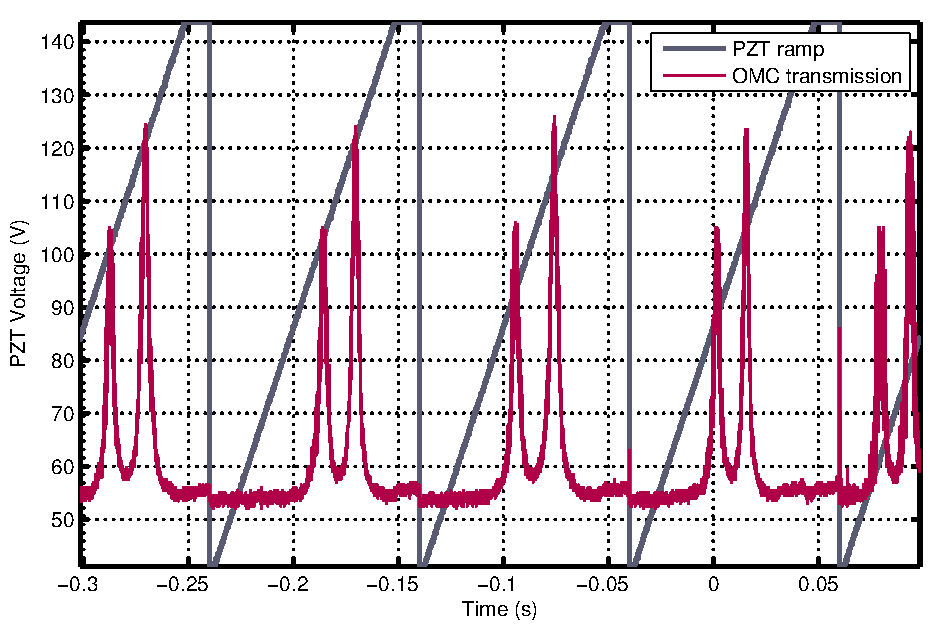
\includegraphics{figs-omc/pztdccal.pdf}
  \end{center}
  \caption[Measurement of the OMC PZT actuator calibration.]{Measurement of the OMC PZT actuator calibration. Both the carrier and subcarrier can be seen passing through resonance.}
  \label{fig:pztsweep}
\end{figure}
The PZT length actuator of the OMC was calibrated by applying a voltage to the PZT to sweep the cavity through both carrier and subcarrier resonances. %NL%
The subcarrier frequency offset was chosen to be close to one FSR separated from the carrier. %NL%
The separation was $1\mathrm{FSR}+3.8$MHz. %NL%
In terms of a change in cavity length, this is 14.5nm, which is twice the distance moved by the mirror. %NL%
Given the known frequency separation of the carrier and subcarrier, a determination of the voltage offset between resonances can be used to calibrate the PZT. %NL%
The data taken are shown in Figure \ref{fig:pztsweep}, and the mean offset of the central three ramps is 19.8V. %NL%
Thus the PZT calibration is $\frac{14.5\text{nm}}{2}\frac{1}{19.8\text{V}}=0.37\text{nm}/\text{V}$.


\section{Optical feedback instability in the OMC}
\begin{figure}
  \begin{center}
  \leavevmode
  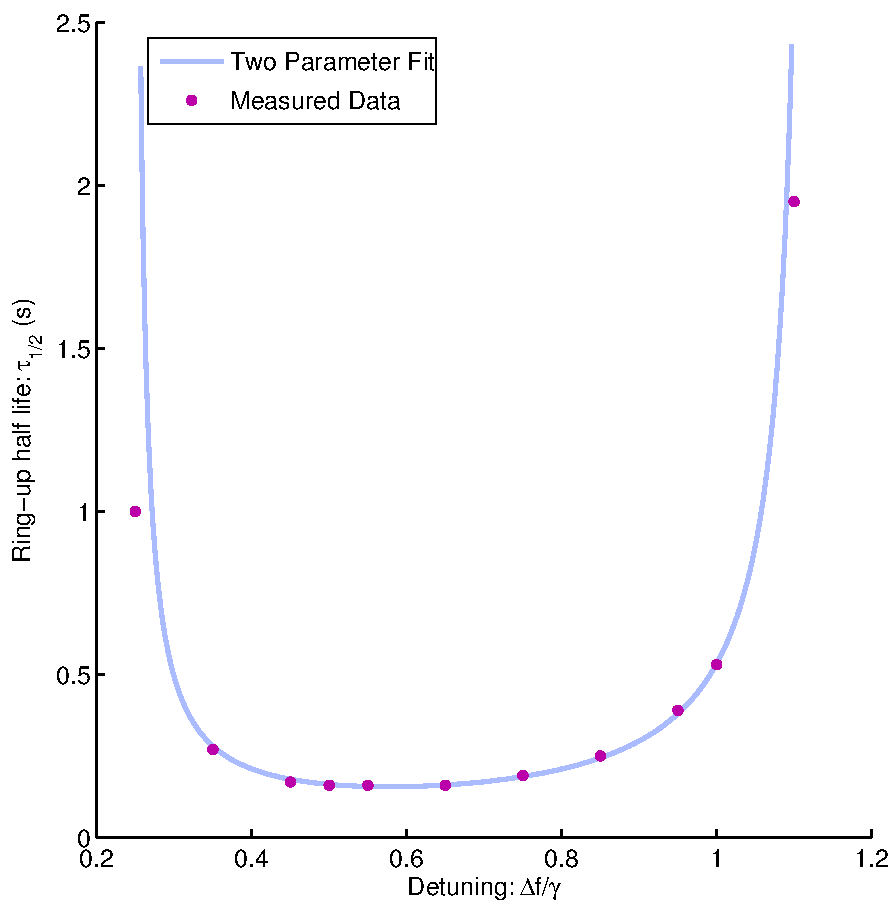
\includegraphics{figs-omc/raddamping.pdf}
  \end{center}
  \caption[Measurement of ring-up times of optical instability in the OMC.]{Measurement of ring-up times of optical instability in the OMC. The instability ring up time was measured for several values of the cavity detuning. Also plotted is a two-parameter curve fit to the data. Data collected by Tim Bodiya and Nicolas Smith-Lefebvre.}
  \label{fig:raddamping}
\end{figure}
An issue arose during Enhanced LIGO which hindered the development of an automatic cavity locking system for the OMC. %NL%
As the OMC was brought into resonance, some kind of dynamical instability would be activated and this would cause signals in the transmitted power at kHz frequencies with amplitudes large enough to saturate the readout electronics. %NL%
Because the locking servo was based on a transmission dither scheme, these instabilities would pollute the cavity length error signal and prevent locking. %NL%
The instabilities would not be excited at the very peak of resonance, so for some fraction of the attempts, there would be a successful lock of the cavity. %NL%
The result of this is that locking the OMC was the only step in the lock acquisition and low noise operation of Enhanced LIGO that was not fully automated during science data taking. %NL%
The lack of an automatic OMC locking system probably had a detrimental effect on the overall duty cycle of the interferometers, but the magnitude of this effect would be difficult to determine.

The mechanism of the instability was never understood. %NL%
It had the following characteristics:
\begin{itemize}
\item The strength of the instability depended on the circulating cavity power. for small power incident on the OMC (less than 1mW) there was no instability.
\item The instability was not coupling through the PZT actuator. The instability remained even with the PZT leads were shorted.
\item There was no instability when the cavity was centered on resonance.
\item There was instability on either side of cavity resonance.
\end{itemize}

There was an attempt to quantify the behavior of this instability by investigating the dependence of the ring-up time of one of the unstable modes with a frequency of 1.1kHz. %NL%
The OMC was locked detuned from resonance with approximately 9mW of power transmitted through the cavity. %NL%
The data that were taken are shown in Figure \ref{fig:raddamping} as the ring-up half life, $\tau_{1/2}$, as a function of cavity detuning, $\Delta f/\gamma$, where $\gamma= \frac{1}{2}\frac{\rm{FSR}}{\mathcal{F}}$ is the cavity linewidth.

Also shown in Figure \ref{fig:raddamping} is a simple model of the ring-up time. %NL%
The model comprises a exponential ring-up characterized by an anti-damping term which has the following functional dependence on the detuning:
\begin{equation}
\label{eqn:gamma}
\Gamma(\Delta f)=\frac{2\Delta f/\gamma}{\left[1+\left(\Delta f/\gamma\right)^2\right]^2},
\end{equation}
which is just the derivative of the cavity transmission profile (Equation \ref{eqn:finesse}) for small $\Delta f$. %NL%
Explicitly, the ring-up half life is
\begin{equation}
\tau_{1/2}=\tau_0\left(\frac{2\Delta f/\gamma}{\left[1+\left(\Delta f/\gamma\right)^2\right]^2}-\Gamma_0\right)^{-1}.
\end{equation}
The best fit of the model to the data is given by $\tau_0=33\pm 6$ms and $\Gamma_0=0.438\pm 0.001$.

Perhaps the most interesting aspect about the model is what mechanism it rules out. %NL%
An opto-mechanical parametric instability driven by radiation pressure would have a third factor of $\left[1+\left(\Delta f/\gamma\right)^2\right]$ in the denominator for Equation \ref{eqn:gamma} \cite{Corbitt:7mK}. %NL%
A curve fit with a model consistent with a radiation pressure instability was also tried, but did not provide a good agreement with the data. %NL%
So although it seems that the instability is somehow driven by the intra-cavity power, it is not consistent with radiation pressure.

Ultimately this did not pose a problem for the noise performance of the interferometer, because the OMC is always kept on resonance during normal operation, it is not operated detuned. %NL%
However, it did remain a poorly understood feature of the system and because Advanced LIGO will use the same, or a similar OMC, it likely warrants further investigation.

\section{OMC performance in Enhanced LIGO and prospects for future interferometers}

The ultimate performance of the interferometer is affected by the OMC in several ways. %NL%
The ability of the OMC to maximally transmit the gravitational wave signal directly affects the shot-noise limited SNR of the interferometer (this is covered in Section \ref{sec:alignsnr}). %NL%
Losses inside the OMC will limit the transmission, but these were shown to be low (Section \ref{sec:omclosses}). %NL%
A more subtle problem is to correctly match the incident beam to the resonant \TEM{00} mode of the OMC, any signal light which is not correctly matched will be rejected. %NL%
From the point of the readout sensitivity, this is effectively a loss. %NL%
The two most common forms of cavity mismatch are alignment (Chapter \ref{ch:beacon}) and mode matching (Chapter \ref{ch:modematching}). %NL%
In addition to signal losses, the addition of an OMC can bring new noise couplings, perhaps the most important being the sensitivity to beam jitter (Chapter \ref{ch:jitter}).

\begin{figure}[h!]
  \begin{center}
  \leavevmode
  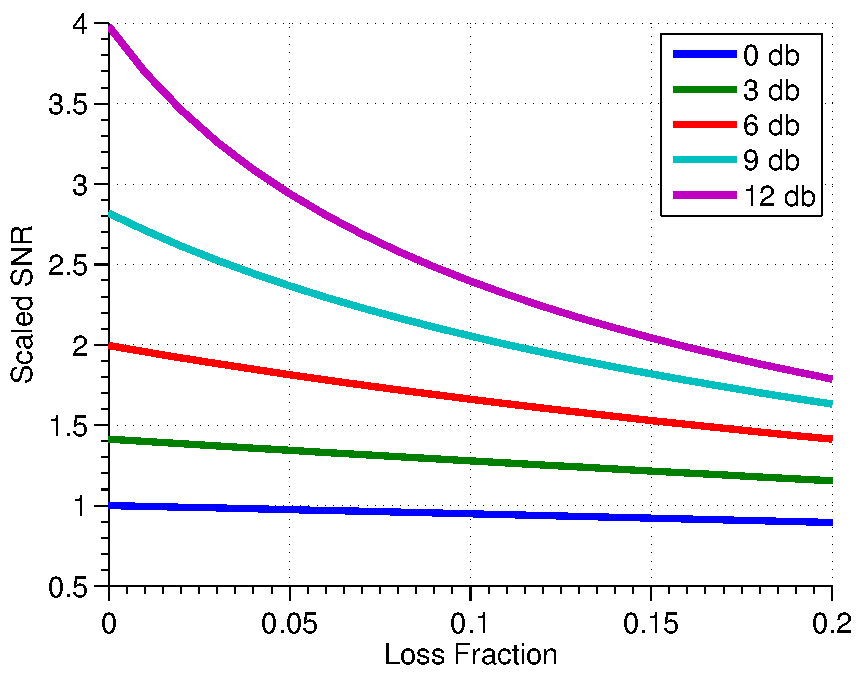
\includegraphics{figs-omc/squeezeplot.pdf}
  \end{center}
  \caption[Interferometer readout SNR gain from squeezing as a function of output losses.]{Interferometer readout SNR gain from squeezing as a function of output losses. Higher levels of squeezing lead to increased sensitivity to output losses, including those from the OMC.}
  \label{fig:squeezeplot}
\end{figure}

An analysis of the readout sensitivity of the two Enhanced LIGO interferometers was performed by \citet{Tobin}. %NL%
This analysis showed that both interferometers performed at the expected level of sensitivity when all known output losses were taken into account. %NL%
The OMCs thus provided the desired outcome of improving the ultimate interferometer sensitivity. %NL%
One of the major sources of loss for the H1 interferometer was mode mismatching, this was the motivation for the system proposed in Chapter \ref{ch:modematching}.

The use of squeezed light to further enhance the readout sensitivity of laser interferometers has recently been demonstrated as both feasible and practical on full scale gravitational wave antennae \cite{GEOSqz:11,LIGOSqz}. %NL%
Output losses become even more important when the interferometer employs squeezed light injection. %NL%
Figure \ref{fig:squeezeplot} shows how losses in the readout chain can degrade the interferometer sensitivity for different levels of squeezed light injection. %NL%
The prospects of squeezing for future interferometers certainly offer great promise for boosting interferometer sensitivity. %NL%
Although, these benefits can only be fully exploited if the output losses are maintained at a minimal level. %NL%
The performance of the OMC is central to realizing these goals.

The following chapter covers some theoretical background necessary for analyzing how the OMC interacts with the output beam of the interferometer.

\chapter{Vector space model of optical systems}
\label{ch:modalmodel}
This chapter describes a formalism that treats the laser field components propagating in an optical interferometer as a complex vector space where common optical components, such as mirrors and optical modulators are treated as operators in this space. %NL%
This treatment allows the analysis of complicated optical paths, which include paths that loop onto themselves (as in the case of resonant cavities) to be reduced to a problem of matrix manipulation. %NL%
This is a powerful technique that is used extensively in modeling the behavior of gravitational-wave interferometers \cite{Vinet1986,Hefetz:97,Sigg:00}, and is useful for some of the concepts discussed in later chapters.

At this point in the discussion, a bird's eye view of the technique is useful. %NL%
In essence what this formalism provides is a significant abstraction and abbreviation of the effects of opical components (mirrors, modulators, etc.) on the the field components that make up a laser beam. %NL%
In the case of the transverse electric-magnetic (TEM) spatial modes of a laser field, a calculation of how a mirror, which is rotated about some axis perpendicular to the beam, redistributes energy from one field component to another may require complicated overlap integrals involving the Hermite-Gaussian profiles of the beam modes. %NL%
Such a calculation is difficult to calculate and and analytical solutions are intractable and unwieldy. %NL%
The strength of this technique is that all of these complicated integrals are \emph{baked in} to the linear operators which represent optical components, so to speak. %NL%
All of the involved integral math is performed in the construction of the operators, and is hidden from view when the optical system as a whole is considered. %NL%
What is left is just a problem of linear algebra.

\section{Frequency components of a laser field}
\label{sec:freqspace}
To get a flavor of the formalism, consider the simple example where we choose our vector space to just have three components that represent the amplitude of a carrier frequency field at frequency $\omega_0$, as well as two sideband fields separated in frequency by $\pm\Omega$. %NL%
Consider an electromagnetic wave propagating in the $z$ direction, at some point along the propagation axis, the electric field at $z=0$ may be written as
\begin{align*}
\geom{E}(t) &= A_0 e^{i\omega_0t}\geom{x} + A_1e^{i(\omega_0+\Omega)t}\geom{x} + A_{-1}e^{i(\omega_0-\Omega)t}\geom{x}\\
&= \left( A_0 + A_1 e^{i\Omega t}+A_{-1}e^{-i\Omega t}\right) e^{i\omega_0 t}\geom{x},
\end{align*}
where $A_0$, $A_1$ and $A_{-1}$ are the carrier, first order upper sideband and first order lower sideband amplitudes respectively, $k=\omega_0/c$ is the wave-number, and $\geom{x}$ is the \emph{geometrical} basis vector pointing along the axis of polarization. %NL%
We are interested in the vector representation where this same propagating field is represented as\footnote{The use of $\doteq$ in (\ref{eq:dotequals}) is meant to convey that the expression on the right side is a representation of the vector on the left side in the chosen vector space. %NL%
The right side of the equation is not written in terms of vectors and thus is not truly equal to the left side.} 
\begin{equation}
\label{eq:dotequals}
\vect{E} \doteq \ms A_0 \\ A_1 \\ A_{-1} \me.
\end{equation}

The basis vectors in this representation are given by the three periodically time varying components of the electric field, namely the carrier, upper and lower sidebands. %NL%
It is important to emphasize that the vectors used in this formalism are in general not simple euclidean vectors, but rather abstract vectors representing different components of the electric field of an electromagnetic wave. %NL%
The inner product of two basis vectors is:
\[
\inprod{r}{s} = \int\limits_{\text{many cycles}}\! \! \! \! \! \! \! \! \!
\dd t \; \: {\left( e^{i\omega_{r}t}\right)^*}e^{i\omega_{s}t} = \delta_{rs},
\]
where $\omega_r$ is the sideband frequency of the $r$th sideband. %NL%
This treatment is analogous to the formalism of quantum mechanics in which the quantum state of a system is defined by a vector in a space spanned by a set of orthonormal basis state vectors. %NL%
In our formalism, the components of the laser field will take the place of the state vectors. %NL%
We will use Dirac bra-ket notation because of this strong analogy.\footnote{One significant difference between quantum mechanics and this formalism is that the quantum state vector of a system must always have unit length, to ensure the state has a probability of 1. %NL%
The length of the vector in this formalism is just a field amplitude, and can take any value.}

Now that we are familiar with using this vector space to represent the desired wave amplitudes, let's examine how we may use an operator to represent some optical component. %NL%
An electro-optic modulator (EOM) can act as a phase modulator for a laser field when a voltage is applied. %NL%
When a periodic signal is applied at frequency $\Omega$, given an input field amplitude $Ae^{i\omega_0 t}$ (ignoring the $z$ dependence) the output amplitude is
\newcommand{\gammahalf}{\frac{i\Gamma}{2}}
\begin{equation}
\label{eq:inputfield}
Ae^{i\omega_0 t + i\Gamma \cos{\Omega t}}\approx Ae^{i\omega_0 t}\left(1+\gammahalf e^{i\Omega t}+\gammahalf e^{-i\Omega t}\right),
\end{equation}
where $\Gamma$ is known as the modulation depth and is assumed to be small. %NL%
One can show that in the example vector space we are considering, this EOM can be represented as the following operator
\begin{equation}
\oper{\Phi}(\Gamma) \doteq 
\ms 
1          & \gammahalf & \gammahalf \\
\gammahalf & 1          & 0          \\
\gammahalf & 0          & 1 \\
\me.
\end{equation}
It is then clear that the act of $\oper{\Phi}(\Gamma)$ operating on an input field constructed as the one used in (\ref{eq:inputfield}) gives the desired output field:
\begin{equation}
\vect{E_{output}}=
\oper{\Phi}(\Gamma)\vect{E_{\text{input}}} \doteq \ms 
1          & \gammahalf & \gammahalf \\
\gammahalf & 1          & 0          \\
\gammahalf & 0          & 1 \\
\me
\ms A \\ 0 \\ 0 \me = A \ms  1 \\ \gammahalf \\ \gammahalf \me.
\end{equation}

So far, we have kept our example relatively simple. %NL%
The vector space we have chosen represents only the first order sidebands generated on the carrier frequency. %NL%
Also, we have only expanded the effect of phase modulation to terms linear in $\Gamma$. %NL%
There is, however, no fundamental reason that the analysis cannot be extended to arbitrary precision. %NL%
The number of components of the vector space can be expanded to account for an arbitrary number of higher order sidebands, and the matrix elements used for $\oper{\Phi}(\Gamma)$ can take their exact values. %NL%
The general form of the phase modulation operator is:
\begin{equation}
\oper{\Phi}(\Gamma) = \sum_{r,s=-\infty}^\infty\vect{r} i^{s-r} J_{s-r}(\Gamma) \form{s},
\end{equation}
where $\vect{r}$ is the basis vector representing the $r$th order sideband component (which includes a $e^{ir\Omega t}$ time dependence), and $J_k(x)$ is the Bessel function of the first kind.\footnote{This can be shown using the so-called Jacobi-Anger identity, $e^{ix\cos\theta}=\sum_{k=-\infty}^\infty i^kJ_k(x)e^{ik\theta}$. %NL%
Also, $J_{-k}(x)=(-1)^kJ_k(x)$, thus $\oper{\Phi}(\Gamma)$ is symmetric.} The ability to calculate to arbitrary precision will continue to hold true when we expand the treatment to include other components of a propagating laser field, such as the transverse spatial modes. %NL%
As long as the solutions are converging, the precision is only limited by the choice of when the vector space is truncated, i.e.\ to what order the calculation is taken.

\section{The modal space}
\label{sec:modalspace}
So far our example prescribes an elegant way to deal with optical components (e.g.\ the modulator) which transfer energy from one component of the electric field (the carrier) to other components (the sidebands). %NL%
This type of approach is also applicable to the components of the electric field corresponding the the transverse spatial modes of the beam, as shown by \citet{Hefetz:97}.

When the paraxial approximation applies it is possible to expand the electromagnetic field into a superposition of modes represented by a Gaussian function of the transverse coordinate, multiplied by polynomials. %NL%
Common choices for the polynomial functions are the Hermite or Laguerre polynomials \cite[Chap. %NL%
16]{Siegman}. %NL%
This formalism associates the modal components with eigenmodes of what is described as the ``perfectly aligned and undistorted optical path''. %NL%
In other words, this formalism describes how the introduction of misalignments and beam distortions alter a laser beam propagating in the system by treating misalignments (or higher order beam distortions) as matrix elements which transfer energy between different spatial modes. %NL%
The misalignments are generally treated as small, and thus, the operators of the optical components differ from the identity operator by small corrections. %NL%
The misaligned solutions of beam propagation are thus treated as perturbations of the aligned solutions. %NL%


The treatment of modes in this formalism is slightly novel due to the fact that, normally, some fundamental Gaussian laser mode is defined to have a particular beam waist $w_0$, and a focused beam with a different beam waist can be written as a series of higher order components with the original beam waist $w_0$. %NL%
In this formalism, the fundamental Gaussian mode may have a beam waist value that changes due to the presence of a lens, but the beam on both sides of the lens would be represented by the same modal state vector (modulo some phase rotation due to propagation). %NL%
It is only the presence of misalignments and distortions that cause significant off-diagonal matrix elements.

Choosing the common Hermite-Gaussian basis, we can use basis vectors which are separable into the mode order of the beam along the $x$ and $y$ transverse axes of the beam. %NL%
A general field vector can be decomposed in the modal space as
\begin{equation}
\vect{E} = \sum_{m,n=0}^\infty A_{mn}\vect{mn}\doteq\sum_{m,n=0}^\infty A_{mn}U_m(x,z)U_n(y,z)e^{-ikz},
\end{equation}
where $U_m(x,z)$ is the $m$th 1-D Hermite-Gaussian mode (for example, as defined in \citet{Siegman}.) The basis modes are also referred to as the Transverse Electric and Magnetic modes of order $mn$ (\TEM{mn}). %NL%
The Hermite-Gaussian modes form a complete orthonormal set of basis functions, therefore the inner product is $\inprod{mn}{kl}=\delta_{mk}\delta_{nl}$.

In the modal space, a simple example operator would be a mirror that has been tilted by an angle $\theta_x$ about the y axis. %NL%
Due to the mirror misalignment, the phase of the beam at the plane of the mirror has been advanced on one side and retarded on the other side, relative to the aligned beam. %NL%
This can be represented as a phase multiplication of $\exp[-2ik\theta_x x]$. %NL%
\citet{Hefetz:97} show that in the modal basis this is satisfied by the operator
\begin{equation}
\oper{M}(\Theta_x) = \exp\left[ -i\Theta_x\sum_{m,n,k,l=0}^\infty \vect{mn} \delta_{nl} \left( \sqrt k \delta_{m[k-1]}+\sqrt m \delta_{m[k+1]} \right) \form{kl}\right],
\end{equation}
where $\delta_{mn}$ is the Kroneker delta; and $\Theta_x = \theta_x \pi w(z)/\lambda$ is the normalized misalignment angle for beam width $w(z)$ and wavelength $\lambda$, at the beam waist, this is the ratio of the misalignment angle to the beam divergence angle. %NL%
One can see that the $k$ index is connected to the $m$ index that differs by one mode number, this will provide the correct transfer of energy from the \TEM{00} mode to the \TEM{10} mode as discussed above. %NL%
We can use a matrix representation with three components representing the \TEM{00}, \TEM{10} and \TEM{01} amplitudes, explicitly for field $\vect{E}$:
\begin{equation}
\vect{E} \doteq \ms \inprod{00}{E} \\ \inprod{10}{E} \\ \inprod{01}{E} \me
\end{equation}

In this representation, 
\begin{equation}
\label{eqn:mirrortilt}
\oper{M}(\Theta_x) \doteq \exp \left( -i 
\ms 
0 & \Theta_x & 0 \\
\Theta_x & 0 & 0 \\
0 & 0 & 0 
\me
\right)
\approx
\ms
1-\frac{1}{2}\Theta_x^2 & -i\Theta_x& 0 \\
-i\Theta_x & 1-\frac{1}{2}\Theta_x^2& 0 \\
0 & 0 & 1 \\
\me .
\end{equation}
The last approximation being valid for small $\Theta_x$,\footnote{Note that $\theta_x$ being small is also required by the paraxial approximation.}
So for small misalignments, the effect of rotating a mirror is to take energy from the \TEM{00} component of the field, and transfer it to the \TEM{10} component, the opposite also being true when the initial field already has a non-zero \TEM{10} component. %NL%
It is also useful to note that the resulting \TEM{10} field has a quadrature which is rotated by $\pi/2$ with respect to the initial \TEM{00} field. %NL%
Or in other words, the amplitude of the \TEM{10} field is in the \emph{phase direction} relative to the \TEM{00} amplitude.

\section{The combined vector space}
To treat the general problem of laser fields propagating through an optical system, it will be useful to consider both frequency and modal components simultaneously. %NL%
This combination was covered in detail by \citet{Sigg:00}.

Mathematically, the combined space is a tensor product of the spaces discussed above. %NL%
The resulting basis vectors will be labeled by four indices, two from the modal space, one from the frequency space, and for completeness, a final index to represent the polarization. %NL%
We can use the following notation for the basis vectors:
\begin{equation}
\vect{mn;r;p}=\vect{mn}_{\text{modal}}\otimes\vect{r}_{\text{frequency}}\otimes\vect{p}_{\text{polarization}}.
\end{equation}
It is understood that the electric field represented by one of these basis vectors is
\[
\vect{mn;r;p} \doteq e^{\left[ i\left( \omega_0+\omega_r\right)t\right]} U_{mn}\geom{\epsilon}_p,
\]
where $\omega_r$ is some mapping from the index $r$ to a set of frequencies; $U_{mn}$ is shorthand for $U_m(x,z)\times U_n(y,z)$; and $\geom{\epsilon}_p$ for $p\in \{1,2\}$ are the polarization unit vectors in the $x$ and $y$ direction, respectively. %NL%
Note that this treatment handles sidebands slightly different from how they are handled elsewhere. %NL%
For example, \citet{Sigg:00} treat radio frequency modulation sidebands differently from audio frequency sidebands, and also only treat audio frequency sidebands which are regularly spaced. %NL%
Using the treatment outlined here in which all sidebands are treated in the same way and may have arbitrary spacing, we are able to more simply investigate cross modulation products of several modulation sidebands, as well as situations where signal detection frequencies are comparable to modulation frequencies. %NL%
This is accompanied by the sacrifice of potentially having many more matrix elements.

An example of an operator in the combined space is the free space propagation operator:
\begin{align}
\label{eq:Propagator}
\oper{P}(\Delta z,\eta) = & \\
\sum_{\substack{mnkl\\rs\\pq}}& \vect{mn;r;p}
\delta_{mk}\delta_{nl}\delta_{rs}\delta_{pq}
\exp  \left[i(m+n+1)\eta
-i\frac{\omega_0+\omega_r}{c}\Delta z\right] 
\form{kl;s;q}, \notag
\end{align}
using parameters
\begin{align*}
\Delta z &= z_{\text{end}}-z_{\text{start}} \\
\eta &= \arctan \left( \frac{(z_{\text{end}}-z_0)\lambda}{\pi w_0^2}\right)- 
        \arctan \left( \frac{(z_{\text{start}}-z_0)\lambda}{\pi w_0^2}\right)
\end{align*}
for starting and ending positions $z_{\text{start}}$ and $z_{\text{end}}$, where $z_0$ is the position of the beam waist, and $w_0$ is the beam radius at the waist. %NL%
The parameter $\eta$ is commonly referred to as the Gouy phase shift. %NL%
As one can see by the presence of the Kronecker deltas in (\ref{eq:Propagator}), all the components of the input field are directly propagated to the output field without mixing. %NL%
There is, however a phase shift which depends on the transverse mode order (the Gouy shift) and the wavelength ($\omega_r/c$).

More complicated operators exist which simultaneously mix mode and frequency components. %NL%
One example is that of a mirror which is dithered at a given frequency in angle. %NL%
It is in a sense a combination of the misaligned mirror operator in section \ref{sec:modalspace} and the phase modulation operator in section \ref{sec:freqspace}. %NL%
This operator is derived by \citet{Sigg:00}.
\section{Photodetection}
A photodetector is a device which is sensitive to the power in the laser field. %NL%
This is typically photodiode which converts the laser power into an electric current. %NL%
In terms of the electric field we may write the time averaged power incident on a photodiode as
\begin{equation}
\bar{P}=\frac{\epsilon_0 c}{2}\int \! \! \dd t \int \! \! \dd A|E^2|=\frac{\epsilon_0 c}{2}\inprod{E}{E}.
\end{equation}
This fits nicely into our formalism because one can view the average power detected at a photodiode as the squared-norm of the state vector of the laser field. %NL%
Often, however, one may use a photodetector to measure certain frequency components of the power, as well as information about the spatial distribution of the beam. %NL%
Here we outline how to treat such signals in this formalism.

The time dependent components of the laser power can be thought of as the mixing of different frequency components of the electric field. %NL%
To achieve this in the vector space formalism, we must use an operator which has matrix elements connecting different frequency components. %NL%
For demodulation at frequency $\omega_d$, the  operator takes the form: 
\begin{equation}
\label{eqn:fdemodoperator}
\oper{D}(\omega_d) = \sum_{rs} \vect{r} \delta(\omega_r,\omega_s-\omega_d) + \delta(\omega_r,\omega_s+\omega_d)\form{s},
\end{equation}
where we use a delta function defined as
\begin{equation}
\delta(\alpha,\beta) = 
\begin{cases}
0 & \text{if $\alpha \neq \beta$}, \\
1 & \text{if $\alpha = \beta$}.
\end{cases}
\end{equation}
Note that there is a special case where $\omega_d=0$ where $\oper{D}(\omega_d)$ is the identity operator, which does not follow from Equation \ref{eqn:fdemodoperator} and must be handled seperately.
\begin{figure}
  \begin{center}
  \leavevmode
  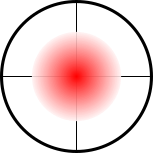
\includegraphics{figs-modalmodel/QPD.pdf}
  \end{center}
  \caption[Diagram of a quadrant photodiode]{Diagram of a quadrant photodiode. The beam is pictured centered on the diode. As the beam is displaced vertically, more photocurrent will be measured by the top two segments than the bottom two. Subtracting the bottom photocurrents from the top ones will provide a measurement of the vertical beam position.}
  \label{fig:QPD}
\end{figure}
Photodetectors are sometimes split into many segments, such as is the case with a so called quadrant photo-detector (QPD). %NL%
In the case of a QPD, the face of the photodetector is split into four equal segments as seen in figure \ref{fig:QPD}. %NL%
Different linear combinations of the photocurrents of these segments can yield different information about the laser beam. %NL%
For example, the vertical displacement of a beam can be determined by subtracting current of the top segments from the bottom segments.

The shape and linear combination of the photodiode segments is treated in the literature\cite{Hefetz:97} as a pupil function $p(x,y)$,  where the photodiode measures a signal
\begin{equation}
S=\frac{\epsilon_0 c}{2}\int \! %NL%
\! %NL%
\dd t \iint\limits_{\text{PD area}}E^\dagger(x,y)p(x,y)E(x,y)\dd x \dd y,
\end{equation}
so for example for a photodetector split along the $y$ axis, $p(x,y)=1$ for $x>0$ and $-1$ for $x<0$.

% show how this is equivalent to an operator

In the language of transverse spatial modes, a split photodetector is measuring the mixing of the \TEM{00} mode with the \TEM{10} mode.\footnote{More precisely, it measures the mixing of all even modes to odd modes and vice versa, with the primary contribution coming from the modes which differ by one mode order.} So in order to model this in the vector space framework, we will need to generalize the demodulation operator to have matrix elements between spatial modes as well as frequency components. %NL%
So we may expand the demodulation operator to include spatial components. %NL%
The spatial matrix elements of the demodulation operator are:
\begin{equation}
\label{eqn:spacedemod}
\matrixel{mn}{\oper{D}(\Omega)}{kl}=\iint\limits_{\text{PD area}}U_{mn}^\dagger(x,y)p(x,y)U_{kl}(x,y)\dd x \dd y,
\end{equation}
where the ``variable'' %NL%
$\Omega$ is just supposed to contain all the information of the pupil function.\footnote{$\Omega$ does not represent an angular frequency in this case.}

The frequency, spatial, and polarization parts of the demodulation operator and combined simply with a tensor product,
\begin{equation}
\oper{D}(\Omega,\omega_d) = \oper{D}(\Omega)_{\text{modal}}\otimes\oper{D}(\omega_d)_{\text{frequency}}\otimes\oper{I}_{\text{polarization}},
\end{equation}
where $\oper{I}$ is the identity operator.

Once the demodulation operator is constructed, the signal measured by the photodetector is
\begin{equation}
S=\frac{\epsilon_0 c}{2}\matrixel{E}{\oper{D}(\Omega,\omega_d)}{E}.
\end{equation}
In terms of the quantum mechanical analogy, the signal measured on a photodetector is just the expectation value of it's demodulation operator.

\section{Vector space model of the output mode cleaner}
The true utility of this formalism arises when the optical system contains paths that branch and loop onto themselves, as is the case with resonant cavities. %NL%
The fact that the operators can simultaneously handle the transverse modes and frequency components reduces much of the complexity of the problem through abstraction.
\begin{figure}
  \begin{center}
  \leavevmode
  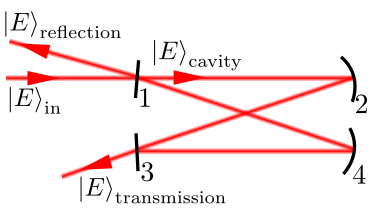
\includegraphics{figs-modalmodel/omcmodal.pdf}
  \end{center}
  \caption[Diagram of vector space model of the OMC]{Diagram of vector space model of the OMC}
  \label{fig:omcmodal}
\end{figure}
%a simple ring cavity
In figure \ref{fig:omcmodal} we see a schematic diagram of a four mirror ring cavity. %NL%
Every interaction of the laser field is handled by an operator. %NL%
This includes transmission through an optic, reflection from an optic, and propagation through free space. %NL%


We may write down an expression for the field inside the cavity as follows
\begin{equation}
\vect{E}_{\text{cavity}} = \oper{T}_1\vect{E}_{\text{input}}+\oper{G}\vect{E}_{\text{cavity'}}.
\end{equation}
Here, $\oper{G}$ is the operator representing one full round trip through the cavity, starting with the propagation from mirror 1 to mirror 2, $\oper{T}_1$ is the operator for transmission through mirror 1, and $\vect{E}_{\text{cavity'}}$ is the cavity field due to the previous round trip of the light. %NL%
When the system has reached a stationary state, $\vect{E}_{\text{input}}=\vect{E}_{\text{cavity'}}$.\footnote{Note that this does not only include fields static in time, but also any peiodically changing fields that are represented in our vector space.} In this case we may solve for the field in the cavity:
\begin{equation}
\vect{E}_{\text{cavity}} = \left(\oper{I}-\oper{G}\right)^{-1}\oper{T}_1\vect{E}_{\text{input}}.
\end{equation}
The round trip operator is 
\begin{equation}
\oper{G} = \oper{P}_{1\rightarrow 2}\oper{M}_2\oper{P}_{2\rightarrow 3}\oper{M}_3\oper{P}_{3\rightarrow 4}\oper{M}_4\oper{P}_{4\rightarrow 1}\oper{M}_1,
\end{equation}
where $\oper{P}_{j\rightarrow j+1}$ is the free space propagation operator from mirror $j$ to $j+1$, and $\oper{M}_k$ is the reflection operator for mirror $k$.

By definition, the mirror operators are all diagonal when the system is aligned. %NL%
Also the propagation operators are diagonal by construction. %NL%
The diagonal matrix elements of $\oper{G}$ vary in their phase from one field component to the next. %NL%
Thus one can see that when these matrix elements have a phase close to an integer multiple of $2\pi$, the cavity field of those components will be enhanced. %NL%
This is of course just the expected resonance behavior. %NL%
As the length of the cavity is changed (which modifies the propagation operators) different field components will come in and out of resonance. %NL%
This includes both frequency components and higher order mode components, indeed different frequency components of different higher order mode components as well!

The following chapter describes an alignment system designed to measure the spatial modes of only a particular frequency component of the laser field. %NL%
The concepts introduced in this chapter are well suited to describe such a system.

\chapter{Optimal alignment sensing of an output mode cleaner}
\label{ch:beacon}
One surprise that arose from the Enhanced LIGO project was the difficulty of OMC alignment. %NL%
During the project, it was learned that the very reason to desire an OMC, e.g.\ the presense of higher order mode (HOM) junk light, is also a source of contamination for a system to correctly align the laser beam into the OMC. %NL%
This chapter describes what ultimately became the solution to that problem.

A critically coupled optical cavity can attenuate the HOM content of a laser beam. %NL%
Such cavities also act as temporal filters for reducing laser amplitude and phase noise for frequencies above the cavity linewidth. %NL%
When such mode cleaner filter cavities are placed at the output (readout) port of an optical system, deriving error signals to control the length and alignment of the Output Mode Cleaner (OMC) cavity poses a particular challenge. %NL%
The signal-rich optical field may be weak compared to the HOM components. %NL%


In this chapter we describe a solution to the problem of aligning the OMC cavity. %NL%
Though we consider the LIGO optical readout here, our scheme applies to any optical system where a signal is encoded as an amplitude modulation of a laser field, and the spatial mode of the signal-induced modulation sideband differs from that of the DC carrier field. %NL%
 In the case of LIGO, the signal is a gravitational wave induced modulation of the optical field, typically at frequencies 10 Hz to 10 kHz shifted from the carrier. %NL%


\section{The alignment problem in a mode cleaner cavity}
%
Fig. %NL%
\ref{fig:beaconblockdiag} shows a schematic representation of the readout system we consider. %NL%
The laser beam incident on the OMC comprises a carrier field and signal sideband fields which must be aligned to the OMC cavity. %NL%
In the absence of technical noise sources, an automatic alignment system should maintain the cavity alignment that maximizes the SNR of the detected signal with respect to the photon shot noise. %NL%
In general the carrier and sideband fields do not occupy the same spatial modes and their transmission through the OMC varies differently as a function of the input alignment. %NL%


As a simple example, consider a beam reflected from an over-coupled Fabry-Perot cavity (OC). %NL%
The OC is held slightly offset from resonance such that periodic length excitations cause amplitude modulation that can be detected on a photodetector. %NL%
Consider the case of a static misalignment of the input carrier field. %NL%
The reflected carrier field will also be misaligned, while the signal field, being generated inside the OC, will be in the same spatial mode as the OC. %NL%
Thus the carrier and signal fields will have a relative misalignment. %NL%
In this example, the cause of the alignment mismatch is a misalignment of the input field to the OC. %NL%
However, in more complicated cases, such as in the case of a LIGO detector composed of multiple, coupled cavities, the source of extra modal content may not be so easily removed.

Consider a carrier field with transmitted amplitude $c$ and amplitude modulated upper and lower signal sidebands fields with transmitted amplitudes $s$. %NL%
The shot noise limited SNR of the signal when measured on a photodetector is proportional to
%
\begin{equation}
SNR \propto \frac{cs}{\sqrt{c^2 + 2s^2}} \approx s.
\end{equation}
%
Here we have made the following simplifying assumptions: the carrier field amplitude is much greater than that of the signal field, the signal fields are pure amplitude modulation, and that there is perfect spatial overlap of the carrier and the sidebands after transmission through the OMC. %NL%
We see that the alignment system that maximizes optical SNR of fields detected after transmission through an OMC simply maximizes the amplitude transmission of the {\it signal field} through the OMC. %NL%
In considering SNR, this chapter only considers shot noise. %NL%
Another important noise source involved with OMC alignment is beam jitter noise, described in Chapter \ref{ch:jitter}.

To leading order, typical alignment schemes sense the ${\rm TEM}_{01}$ and ${\rm TEM}_{10}$  modes of the carrier field measured in the the OMC eigenmode basis\cite{Anderson1984}. %NL%
The presence of these modes is interpreted as a misalignment. %NL%
In this chapter we will show how to modify a common alignment technique to be sensitive to signal field misalignments, and thus allow one to maximize the SNR of the signal.

\begin{figure}%[placement t]
  \begin{center}
  \leavevmode
  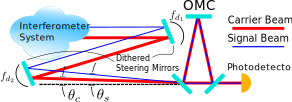
\includegraphics{figs-beacon/blockdiagtight.pdf}
  \end{center}
  \caption[Block diagram of dither alignment sensing.]{A signal is encoded by interferometry (or any other means) as an amplitude modulation of a laser beam. The beam is then steered by two mirrors which are dithered in angle before passing though a mode cleaner cavity. Alignment signals can be derived by demodulation of the transmitted photocurrent. The misalignment has been grossly exaggerated in the figure.}
  \label{fig:beaconblockdiag}
\end{figure}

Consider a single alignment degree of freedom where misalignments of the carrier and the signal fields are represented by one set of misalignment angles $\theta_c$ and $\theta_s$. %NL%
Dither alignment sensing is commonly achieved by mechano-optical modulation of an angular degree of freedom, e.g by driving steering mirrors that direct the beam into the OMC, as shown in Fig. %NL%
\ref{fig:beaconblockdiag}. %NL%
Each mirror is dithered in angle with constant amplitude at a given frequency to modulate the input pointing into the cavity. %NL%


Figure \ref{fig:ditherarrows} shows the frequency content of the field transmitted through the OMC. %NL%
The carrier field is separated in frequency from two amplitude modulated signal sideband fields at $\pm f_b$. %NL%
The dithering steering mirror produce two sidebands at $\pm f_d$, with a field amplitude proportional to $\theta_c$ (alternatively, the ${\rm TEM}_{01}$ mode amplitude\cite{Sigg:00}). %NL%
The signal field also has dither sidebands proportional to $\theta_s$. %NL%
The demodulated signal is made of products of field amplitudes separated by the demodulation frequency.

We will use the notation $P(f)$ to represent the OMC transmitted photocurrent demodulated at the frequency $f$. %NL%
We define the standard dither alignment signal as
%
\begin{equation}
\label{eq:sstandard}
S_{standard} = P(f_d) \propto 2c^2 \theta_c + 4 s^2 \theta_s \approx 2c^2 \theta_c,
\end{equation}
%
where $c$ is the carrier field amplitude, $s$ is the signal field amplitude. %NL%
For the case where the carrier power is much greater than the signal field power ($c^2 \gg s^2$), the demodulated alignment signal is sensitive only to misalignments of the carrier field. %NL%
{\it In this scheme the error signal is nulled at an alignment where the total transmitted cavity power is maximized.} We will refer to this as the {\it standard dither scheme}.

%
\begin{figure}%[placement h]
  \begin{center}
  \leavevmode
  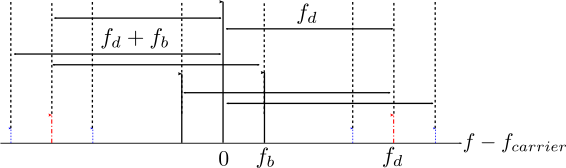
\includegraphics{figs-beacon/ditherarrows.pdf}
  \end{center}
  \caption[Arrow diagram of dither alignment signals.]{Arrow diagram showing electric fields after transmission through the OMC. In the figure, $f_d$ is the angular dither frequency, $f_b$ is the beacon modulation frequency.}
  \label{fig:ditherarrows}
\end{figure}
%

\section{``Beacon'' alignment sensing}
\label{sec:beaconalignment}

To better sense the alignment of the signal field one may create a large amplitude modulation of the signal, say by modulating the length of the signal cavity. %NL%
This modulation creates a frequency tag of the spatial mode of the signal field. %NL%
We refer to this as a ``beacon'' %NL%
modulation, and $f_b$ is the modulation frequency.

As in the standard dither scheme, steering mirrors are used to dither the angle of the beam. %NL%
The desired error signal in this scheme is produced by demodulating the transmitted power at $f_b+f_d$ or $f_d-f_b$, or the sum of these signals. %NL%
We define the beacon alignment signal as
%
\begin{equation}
\label{eq:sbeacon}
S_{beacon}=P(f_d+f_b) \propto 2sc\theta_c+2cs\theta_s.
\end{equation}
%

When this error signal is nulled, the SNR is improved in comparison to standard dither, but sensitivity to the carrier field remains, so the SNR will not be maximized. %NL%
Because the beacon modulation is small, $S_{beacon}$ will have a higher relative noise level than the standard dither approach.

\section{Experimental Demonstration of Beacon Alignment Sensing}
%


The beacon alignment scheme was compared directly to a standard dither scheme using the OMC cavity at the output of the 4 km LIGO Interferometer at Hanford (H1). %NL%
The readout was arranged as in Fig. %NL%
\ref{fig:beaconblockdiag}. %NL%
The angular dither frequencies were between 1.5 and 2.5 kHz, while the beacon modulation was a 10 Hz excitation of the differential arm length. %NL%


The differential arm length of the interferometer is sensed as an amplitude modulation at the output port. %NL%
The static carrier at the antisymmetric port is generated by an offset of the differential arm length. %NL%
The OMC filters the spatial and frequency content of the beam before the beam is split equally and detected on two photodetectors. %NL%
The LIGO interferometers are examples of optical systems where a beacon based alignment system performs significantly better than a standard dither scheme. %NL%


%
\begin{figure}
  \begin{center}
  \leavevmode
  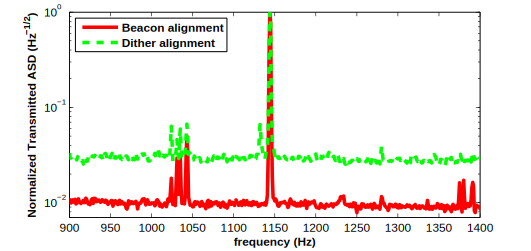
\includegraphics{figs-beacon/shotSNRtightedited.pdf}
  \end{center}
  \caption[An instance of the noise performance of beacon alignment sensing.]{The noise amplitude spectral density of the LIGO H1 detector using two types of alignment schemes. The curves are normalized to a calibration line at 1144 Hz.  The small line structures are resonances of the suspension wires supporting the mirrors. The beacon scheme shows an SNR improvement of about a factor of 3.}
  \label{fig:shotnoise}
\end{figure}

Fig. %NL%
\ref{fig:shotnoise} shows the amplitude spectral density of the transmission of the OMC of the H1 interferometer. %NL%
The plot is centered on an injected calibration signal at 1144 Hz and the curves are normalized to the peak height of this line. %NL%
The calibration line is surrounded by primarily shot noise. %NL%
The dashed green curve (color online) shows the performance using dither sensing, while the solid red curve shows beacon sensing. %NL%
The SNR of the calibration line is improved by about a factor of 3.1 by using a beacon scheme. %NL%
A factor of 2.4 is due to an increase of signal strength and the remaining factor of 1.3 is due to a reduction in the total transmitted power, and hence the shot noise. %NL%
We propose that the poor performance of the standard technique is due to excess HOMs in addition to the ${\rm TEM}_{01}$ mode associated with misalignment.
% talk about HOMs that aren't 10/01?

\section{Optimal alignment sensing of the signal sideband field}
%\label{sec:optimalalignment}
It is possible to combine the standard dither signal with the beacon signal to produce a signal which is sensitive to signal field misalignments only. %NL%
We also make use of the DC transmitted power, $P_{DC} = P(0) \approx c^2$, and the beacon modulation amplitude, $P(f_b) \approx 2cs$. %NL%
An optimal alignment signal can be constructed as follows:
%
\begin{align}
\label{eq:optsig}
S_{optimal} &= S_{beacon} - \frac{P(f_b)}{2P_{DC}} S_{standard}\\
\nonumber &\propto 2cs\theta_s+2sc\theta_c-\frac{2cs}{2c^2}(2c^2\theta_c) \\
\nonumber &\propto 2cs\theta_s.
\end{align}
%

An alternative (though mathematically equivalent) technique would be to just make a dither servo which maximizes the optical SNR directly. %NL%
This may be a more desirable approach depending on how signals are read out and if digital processing is possible. %NL%
In this approach, the SNR should be calculated in real time and demodulated at the dither frequency to provide the error signal.

As above, if the beacon amplitude on the photodetector is $P(f_b)$ and the DC power is $P_{DC}$, the optical SNR is
%
\begin{equation}
SNR = \frac{P(f_b)}{\sqrt{P_{DC}}}.
\end{equation}
%
Any dither sensing scheme is essentially measuring the partial derivative of a signal with respect to the dithered degree of freedom \cite{Kawabe:94}. %NL%
Thus, a dither servo which maximizes the SNR will measure a signal proportional to
%
\begin{equation}
\frac{\partial}{\partial \theta} \left( \frac{P(f_b)}{\sqrt {P_{DC}} } \right) = \frac{1}{\sqrt {P_{DC}}} \left( \frac{\partial P(f_b)}{\partial \theta} - \frac{P(f_b)}{2P_{DC}} \frac{\partial P_{DC}}{\partial \theta} \right),
\end{equation}
%
which is equivalent to (\ref{eq:optsig}) up to constant factors. %NL%
This also shows that this signal is nulled at maximum SNR.

%This is a good place to talk about DARM supressed beacon. 
In gravitational-wave detectors, the OMC transmission is often held constant by a control system. %NL%
If $f_d$ is within the control bandwith, but $f_b$ is not, then the carrier alignment sidebands will be suppressed. %NL%
Sufficient suppression makes the beacon scheme approximately equivalent to the optimal scheme. %NL%
This was the configuration used by both the L1 and H1 interferometers in the sixth LIGO science run \cite{Tobin}.

\section{Generalization of optimal signal-sideband alignment to other alignment sensors}

The technique of using a beacon modulation to sense misalignment of the signal field can be generalized to other types of alignment sensors, for example: split quadrant photodetectors detecting light picked off the beam entering the OMC or split quadrant detectors in reflection of the OMC coupled with frequency or length dithered sidebands, also known as wavefront sensors.

We define the standard carrier alignment signal as $G_{standard}$. %NL%
We also define another signal, demodulated $f_b$ away from the standard signal, as $G_{beacon}$. %NL%
$P_{DC}$ and $P(f_b)$ are defined as in (\ref{eq:optsig}). %NL%
The generalized signal is:
%
\begin{equation}
G_{optimal} = G_{beacon} - \frac{P(f_b)}{2P_{DC}} G_{standard}.
\end{equation}
%
We emphasize that the $G$ signals are derived from the alignment sensor, while the $P$ signals are derived from the OMC transmission.

To summarize, we have introduced the concept of using a beacon as a strong modulation close to signal frequencies to generate alignment signals that lead to increased SNR compared to the standard dither scheme. %NL%
The beacon scheme demonstrates a factor of 3 improvement in SNR for the LIGO H1 detector. %NL%
Finally, we propose a detection scheme to give optimum SNR when used to align an OMC or filter cavity.

\section{Optimal beacon performance in Enhanced LIGO}
\com{fill me!}
\com{talk about Matt's measurement, how much junk 10 is there?}
\com{mention the drum beacon a little too}
\chapter{Techniques for reducing output mode cleaner beam jitter noise}
%This was in my opinion the most important noise source that came with the inclusion of the OMC in LIGO
\com{say how this mechanism doesn't exist without OMC}
% talk about how it was seen by Seiji in 40m cavities, but also by keita with GEO OMC.
\com{Seiji's jitter paper}\cite{Kawamura:94}

\section{The noise mechanism of beam jitter incident on a high finesse cavity}

Motion of the beam incident on a high finesse cavity alters the overlap of said beam with the resonant mode of the cavity. %NL%
This leads to fluctuations in the amount of light which can couple into the cavity and consequently, power fluctuations of the transmitted beam. %NL%
The power fluctuation can spoil the measurement of the intrinsic amplitude modulation of the beam if the measurement and fluctuations occur at the same frequencies.

For a beam incident on the cavity which has a lateral (perpendicular to the direction of propagation) and angular misalignment, constrained to a plane, we have the following expression for the power transmitted through the cavity
\begin{equation}
\label{eqn:simplejitter}
P\approx P_0\left(1-\left(\frac{\Delta x}{w_0}\right)^2-\left(\frac{\theta}{\theta_d}\right)^2\right),
\end{equation}\com{check for factor 2 error, also with modal model chap}
where $P_0$ is the power transmitted of the aligned beam, $\Delta x$ is the beam waist displacement, $\theta$ is the beam waist tilt, $w_0$ is the beam waist radius, and $\theta_d$ is the divergence angle of the beam. %NL%
The approximation holds while both the angular and lateral misalignments are small.

Equation \ref{eqn:simplejitter} shows that beam misalignments couple to the transmitted power quadradically. %NL%
This leads to a few relevant consequences. %NL%
The coupling of beam jitter to transmitted power is nonlinear, thus frequency components of the beam motion may be mixed together, producing new frequencies in the transmitted power. %NL%
Also, the linear coupling coefficient of beam jitter to power fluctuations is proportional to the DC beam misalignment. %NL%
This causes the direct linear coupling of frequency components of beam jitter to power fluctuations to vary as the DC pointing error varies.

Steering optics in the beam path leading to the cavity which are vibrating may transfer vibrations to the laser beam and produce beam jitter noise. %NL%
Let us investigate beam jitter coupling of an optic in the modal picture. %NL%
 We will work in a basis of only the \TEM{00} and \TEM{01} modes. %NL%
Let's assume we have a beam which is dominantly in the \TEM{00} mode as measured in the basis of our cavity, with some small amplitude of \TEM{01} mode. %NL%
In other words, we begin with a beam which is slightly misaligned.
\begin{equation}
\vect{E}_{\text{input}}=E_0\left(\vect{00}+\alpha\vect{01}\right).
\end{equation}
The misalignment, $\alpha$ may be do to another steering mirror upstream, or a misalignment of the beam source relative to our cavity axis, the precise origin is not critical for this discussion.

Now we will assume this beam is incident on a steering mirror before it finally enters the cavity. %NL%
This steering mirror also has a slight misalignment, $\theta$. %NL%
Equation \ref{eqn:mirrortilt} shows the matrix representing the operator of a mirror which has been tilted from nominal alignment. %NL%
The beam incident on the cavity is then
\begin{equation}
\vect{E}_{\text{incident}}=\oper{M}(\Theta)\vect{E}_{\text{input}},
\end{equation}
where, as before, $\Theta=\frac{\theta \pi w(z)}{\lambda}$, while $w(z)$ is the beam width radius at the mirror, and $\lambda$ is the laser wavelength. %NL%
Because the cavity has a high finesse, when the cavity is resonant on the \TEM{00} mode, only that mode is transmitted. %NL%
Thus, for the field transmitted by the cavity
\begin{equation}
E_{\text{t}}=t_{\text{cavity}}\matrixel{00}{\oper{M}\left(\Theta\right)}{E}_{\text{input}}=t_{\text{cavity}}E_0\left(1-i\frac{ \pi w(z)}{\lambda}\theta\alpha\right),
\end{equation}
where \com{finish}. %NL%
This causes a power fluctuation on trasnmission
\begin{equation}
\label{eqn:mirrorjitter}
P=E_t^*E_t=P_0\left(1+\frac{2\pi w(z)}{\lambda}\theta\Im(\alpha)\right).
\end{equation}
\com{calibrated beam jitter meas?}
Only the imaginary part of $\alpha$ contributes to beam jitter noise of our mirror because it represents an error in alignment \emph{angle}, not position, at the location of the steering mirror $\oper{M}$. %NL%
\com{can reproduce first equation with correct definition of alpha}

One interesting consequence of Equation \ref{eqn:mirrorjitter} is that for a given mirror, the strength of beam jitter coupling is proportional to $w(z)$, the size of the beam on the optic. %NL%
Thus one technique for reducing beam jitter coupling is to design one's optical path in such a way that beams are smaller on optics that may produce significant beam jitter. %NL%
This of course also reduces their efficiency as an alignment control mirror.

Futhermore, we again see a nonlinear coupling in the form of mixing of the incident misalignment, $\alpha$, and the jitter of the steering mirror, $\theta$. %NL%
We may suppose that the input alignment has both a DC component and possibly some low frequency (a few to several Hz) wandering motion. %NL%
If this is coupled with high frequency (i.e. %NL%
frequencies in the detection band) jitter of the steering mirror, the mixing of frequencies can cause noise in the power transmission at and around the jitter frequency of the steering optic.

\begin{figure}
  \begin{center}
  \leavevmode
  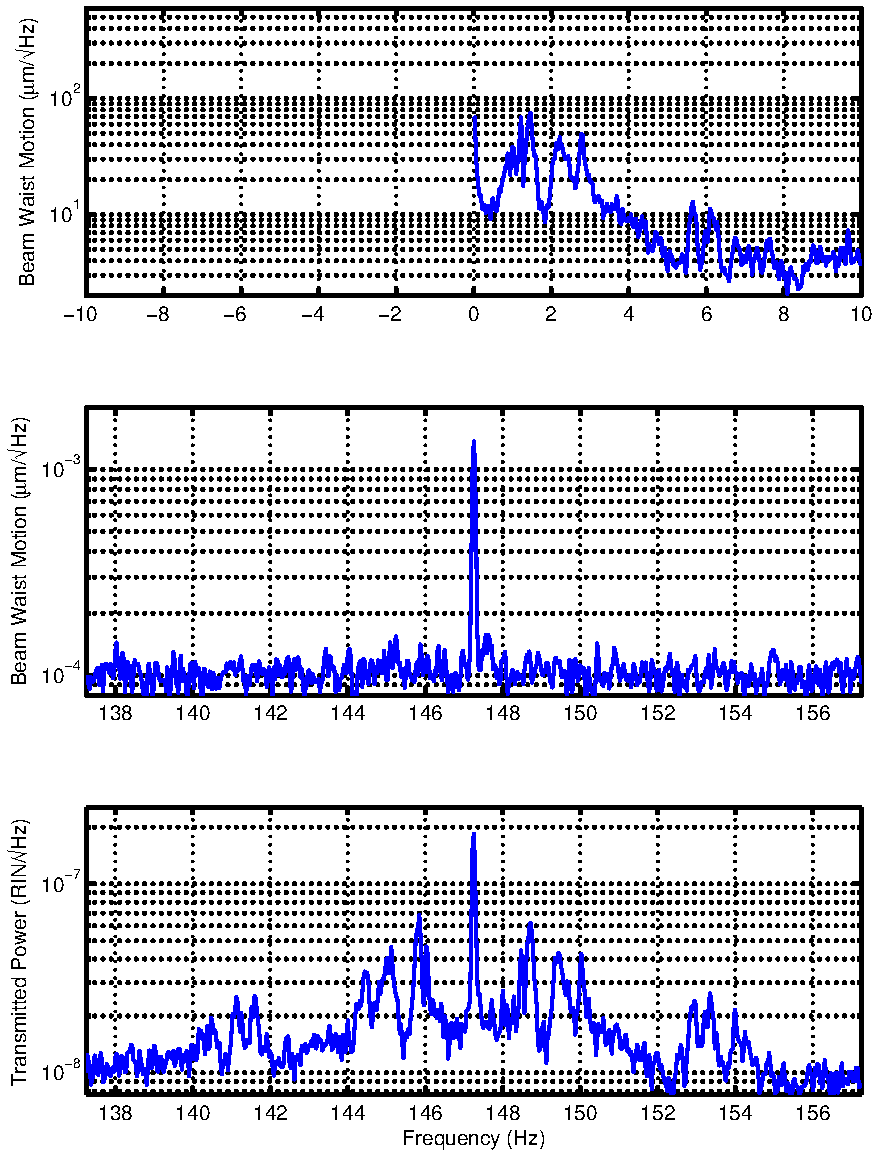
\includegraphics{figs-jitter/bilinearplot.pdf}
  \end{center}
  \caption[Measurement of the bilinear coupling of beam jitter noise.]{Measurement of the bilinear coupling of beam jitter noise. The top panel shows low frequency beam motion measured by the OMC input QPDs. Shown in the center panel is an audio frequency beam jitter peak, this peak was shown to arise from a vacuum scroll pump outside of the HAM6 chamber \cite{robert147}. The bottom panel shows how the low frequency motion has been imparted as sidebands on a central beam jitter peak in the OMC transmitted light. \com{make shorter}}
  \label{fig:bilinear}
\end{figure}

With the introduction of the OMC in Enhanced LIGO, bilinear beamjitter coupling became a much more prominant source of noise. %NL%
Figure \ref{fig:bilinear} shows how low frequency beam motion mixes with high frequency jitter to produce broad sidebands around beam jitter peaks. %NL%
This is similar to how beam jitter was discussed by \citet{Tobin}.

\section{Mechanical resonances of beam steering optics}
When the Enhanced LIGO interferometers were first performing at a sensitivity comparable to the state of the interferometers in the S5 science run, there were large glaring peaks in the sensitivity spectrum. %NL%
It was determined fairly quickly that these were due beam jitter, but the mechanism causing the jitter was unkown.

The Enhanced LIGO upgrade introduced several modifications to the readout chain of the interferometer. %NL%
As discussed in Chapter \ref{ch:omc}, with the introduction of the in-vacuum OMC, it was necessary to use new beam steering and modematching optics to couple the beam exiting the interferometer to the OMC cavity. %NL%
These steering optics, as well as the OMC, were all housed in a single vacuum chamber on top of the prototype HAM ISI platform which is planned to be used copiously in Advanced LIGO. %NL%
Although it was not fully appreciated at the start of Enhanced LIGO, the new isolation platform provided much reduced vibration isolation at audio frequencies when compared to the isolation tables used in the HAM chambers in Initial LIGO. %NL%
Figure \ref{fig:hamtransmission} shows a comparison of the transmission of ground motion to motion of the HAM table for both the initial LIGO passive isolation system, and the Enhanced LIGO HAM ISI.

\begin{figure}
  \begin{center}
  \leavevmode
  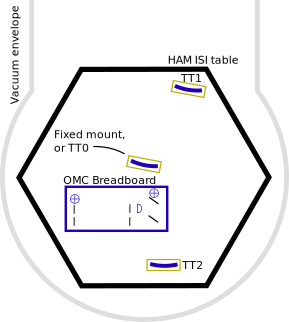
\includegraphics{figs-jitter/ham6layout.pdf}
  \end{center}
  \caption[Schematic of HAM6 optical layout.]{Schematic of HAM6 optical layout. The beam which exits the interferometer antisymmetric port is directed by three steering mirrors onto the OMC. The first steering mirror was originally a fixed post, and changed later to a passive suspended Tip Tilt optic. The second and third Tip Tilts were known used for active beam steering control. A small fraction of the light incident on the OMC transmits through a highly reflective steering mirror and is sensed by two quadrant photodetectors.}
  \label{fig:ham6layout}
\end{figure}

\begin{figure}
  \begin{center}
  \leavevmode
  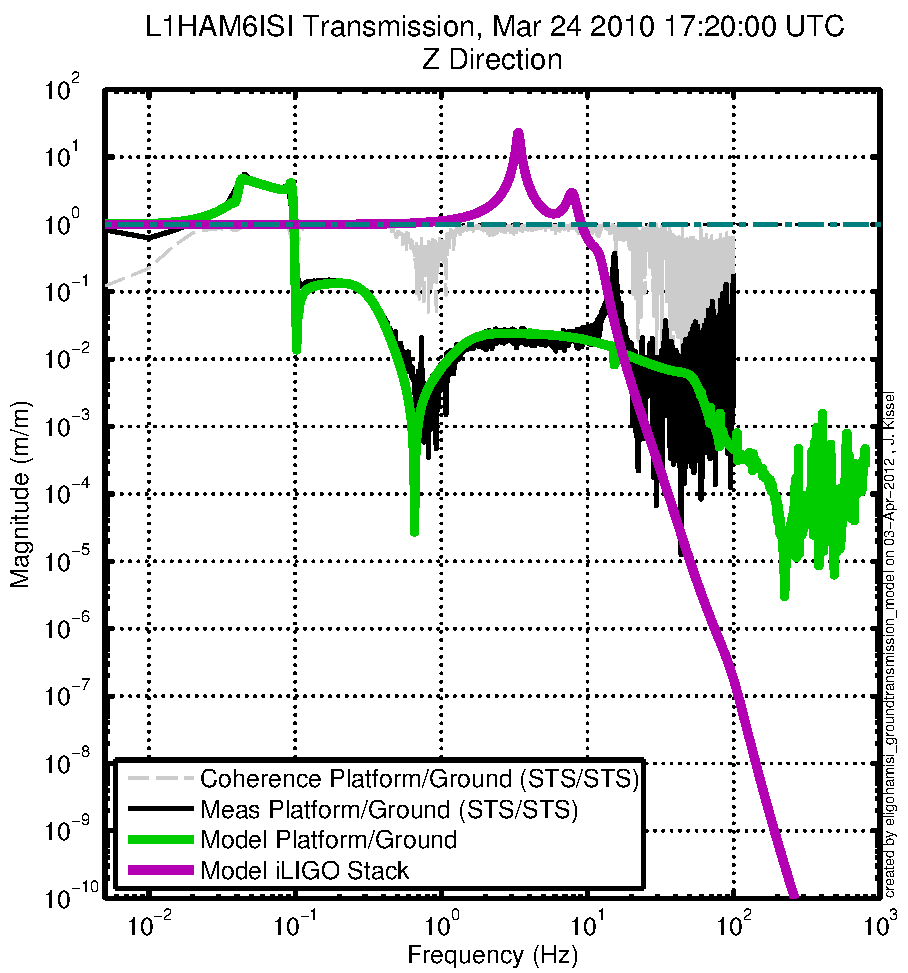
\includegraphics{figs-jitter/hamtransmission.pdf}
  \end{center}
  \caption[Comparison of vibrational motion transmission of the Initial and Enhanced LIGO HAM chamber isolation systems.]{Comparison of vibrational motion transmission of the Initial and Enhanced LIGO HAM chamber isolation systems. While the low frequency isolation of the HAM ISI is far superior to that of the old passive stack, in the most sensitive region of the interferometer (100-200Hz), the HAM ISI transmits a few orders of magnitude greater than the passive system. The high frequency behavior of the HAM ISI model (green curve) represents true resonant structure and is not a result of measurement noise. Credit and appreciation for this figure goes to Jeff Kissel.}
  \label{fig:hamtransmission}
\end{figure}

The optical layout of the OMC chamber of Enhanced LIGO comprised three steering optics, which also behaved as a mode matching telescope, and the OMC itself. %NL%
In the initial configuration, the first of these was a mirror on a fixed mount, while the other two were in a Tip-Tilt suspension system with active beam steering. %NL%
A diagram of the optical layout is shown in Figure \ref{fig:ham6layout}. %NL%
Diligent work by Robert Schofield determined that some of the largest beam jitter peaks degrading the interferometer sensitivity were due to vibrations of the fixed mirror mount \cite{fixedmountpeaks}. %NL%
To rectify this situations, the fixed mirror mount was replaced with a small mirror suspension similar to the Tip Tilts but without the active steering control. %NL%
Comparison of the old and new designs are shown in Figure \ref{fig:TT0photos}. %NL%
This new style was refered to as the passive Tip Tilt, or TT0. %NL%
As seen in Figure \ref{fig:sensimprovement}, this was effective at removing the largest peaks, though some new peaks appeared in the 150-200Hz region.

\begin{figure}
  \begin{center}
  \leavevmode
  \includegraphics{figs-jitter/TT0photos.pdf}
  \end{center}
  \caption[The evolution of the passive Tip Tilt.]{The evolution of the passive Tip Tilt. These photos show several stages in the configuration of the first modematching/steering mirror used in HAM6. The original design was an optic mount attached to a fixed post, shown in the left panel. This was later changed (shown in center panel) to a passively suspended version, made by University of Florida, designed by M. Meyer at LIGO Livingston based on the original active Tip Tilt design. The right panel shows a further re-design where the upper suspension wire clamps are attached by blade springs to the suspension cage.}
  \label{fig:TT0photos}
\end{figure}

The origin of the peaks located in the most sensitive region of the LIGO sensitivity spectrum (``the bucket'') was finally determined by a measurement of the coupling of motion from the table to the pointing of the laser beam itself. %NL%
The OMC was equipped with a pair of quadrant photodetectors (QPDs) which sampled the beam incident on the OMC. %NL%
These QPDs were used to measure the response of the beam motion to motion of the ISI table, which is measured by inertial sensors built into the table. %NL%
A measurement of the transfer function of table motion to beam motion may be seen in Figure \ref{fig:TTbounceTF}. %NL%
The resonances were determined to be the bounce (veritcal) and roll (rotation about the beam axis) modes of the Tip Tilt optics \cite{tt1bounce}.

\begin{figure}
  \begin{center}
  \leavevmode
  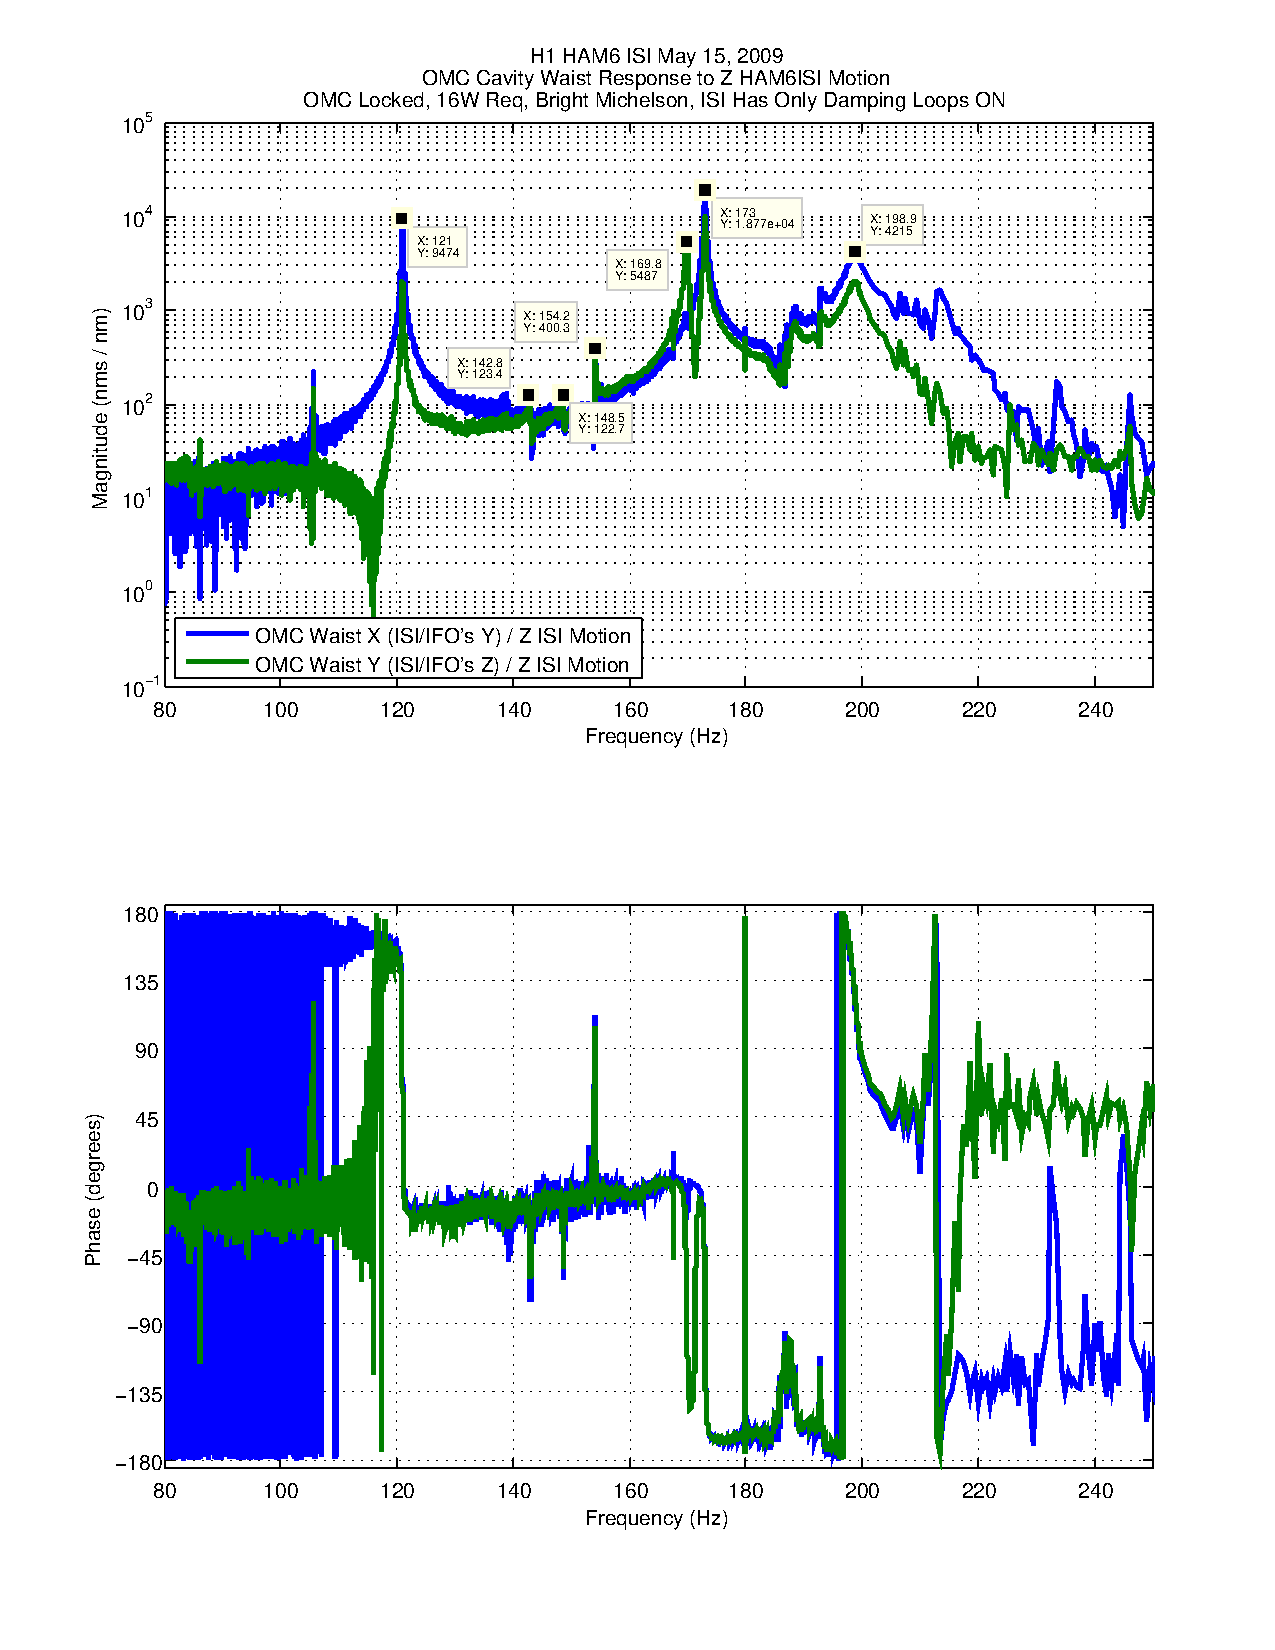
\includegraphics[width=\textwidth]{figs-jitter/TTbounceTF.pdf}
  \end{center}
  \caption[Measurement of HAM table motion coupling to beam motion.]{Measurement of HAM table motion coupling to beam motion. This measurement was performed while all three Tip Tilts used thick suspension wires and no blade springs. This measurement provided evidence that it was the optics on HAM6 which were causing beam jitter peaks in the sensitivity curve of the interferometer.}
  \label{fig:TTbounceTF}
\end{figure}

\begin{figure}
  \begin{center}
  \leavevmode
  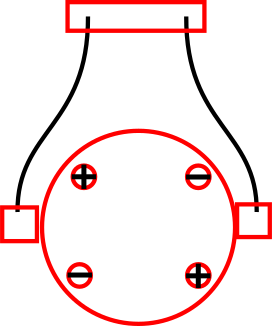
\includegraphics{figs-jitter/ttdiag.pdf}
  \end{center}
  \caption[Diagram of the Tip Tilt suspension with thick wires.]{Diagram of the Tip Tilt Suspension with thick wires. The thickness of the wires caused them to hang with a curve (the curve is exaggerated in this Figure), which lowered the vertical resonance frequency relative to straight wires. Also shown is the relative polarity of the permanent magnets used for active beam steering control.}
  \label{fig:ttdiag}
\end{figure}

The Tip Tilt design had originally assumed the vertical restoring force was due only to strethcing tension in the wires. %NL%
The vertical resonance was expected to lie near the 340Hz violin resonances of the main interferometer test mass suspensions, which were already In fact, the wires had a sufficient gague of \com{big} which caused the break off point of the suspension to be far from the wire clamp. %NL%
This resulted in the wire taking more of an `S' shape than expected, as shown in Figure \ref{fig:ttdiag}. %NL%
The bend in the wire resulted in giving the wire much more yield, reducing the resonant frequencies and placing them directly in the most sensitive region of LIGO. %NL%
A finite element analysis of resonances of optics suspended by curved optics was performed by Matt Evans and supported this general theory \cite{mattfea}.

\begin{figure}
  \begin{center}
  \leavevmode
  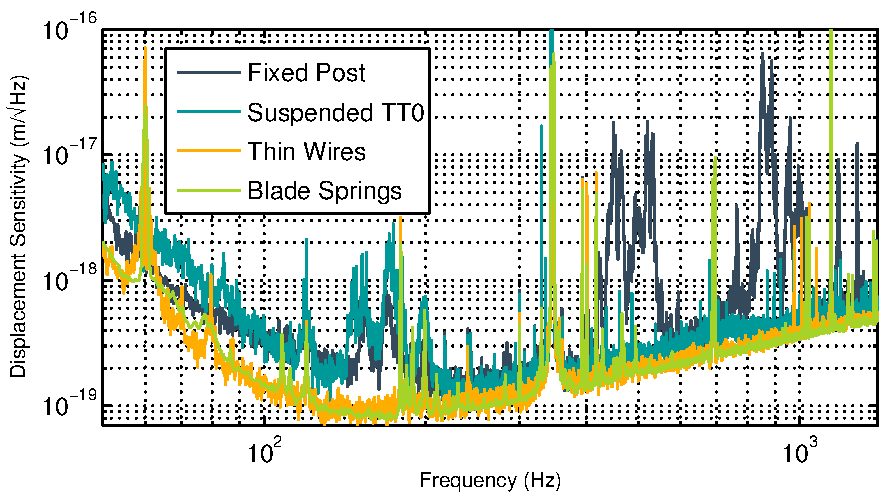
\includegraphics{figs-jitter/sensimprovement.pdf}
  \end{center}
  \caption[Measurement of interferometer sensitivity for different Tip Tilt designs.]{Measurement of interferometer sensitivity for different Tip Tilt designs. Changing the configuration of TT0 from a fixed post to a suspended optic removed large features in the 400-1000Hz region, but increased the noise in the 150-200Hz region. Most features were removed when all Tip Tilts were suspended by thin wires. Finally the configuration was changed again to use blade springs due to the fragility of the thin wires, this also removed the vertical resonance of TT1 near 80Hz. Changes in the background noise floor are not due to modifications of the Tip Tilts. \com{make skinnier.}}
  \label{fig:sensimprovement}
\end{figure}

The Tip Tilt suspension was first modified by using thinner wires of gague \com{small 0.002"}. %NL%
This had the desired effect of reducing the frequency of the bounce resonance to be below the sensitive measurement band \cite{smallwirecoupling}, but could not function as a permanent solution due to the fragility of the wires.\footnote{One of the Tip Tilts doubled as a fast beam diverter to protect the OMC photodiodes from the full stored energy of the arm cavities which exits the AS port when the interferometer loses lock. %NL%
This system would put considerable force on the suspension and after several lock loss cycles it broke one of the Tip Tilt suspension wires.\com{.003" after}} The ultimate solution was to place the upper wire clamps at the ends of blade springs. %NL%
The new Tip Tilt assembly is shown in Figure \ref{fig:TT0photos}. %NL%
This reduced the vertical resonances to near 20Hz \cite{bladebounce,bladebounceLHO}, outside of the sensitive region, but while still allowing the use of wires with enough strength. %NL%
The sensitivity of the interferometer after this change was made is shown in Figure \ref{fig:sensimprovement}. %NL%
Some amount of high frequency acoustic coupling was re-introduced with the blade springs, likely due to strong passive damping of the vertical eigenmodes with Viton rubber \cite{G1100330}, though it was not a limiting noise source.

Mechanical resonances of optic supports in the beam path should stay in the front of the mind of those investigating sources of beam jitter noise. %NL%
Determining the precise source is certainly helped by having the luxury of an optics table equipped with position sensors and an actuation system.
\section{Magnetic field coupling and feedforward subtraction}
Even after the mitigation of mechanical beam jitter on the OMC, there was still significant pollution of the LIGO sensitivity at frequencies surrounding 60Hz. %NL%
60Hz is the frequency of the AC power distribution system in the U.S.A. %NL%
and is a well known source of trouble to those attempting to do precision measurement. %NL%
It is not terribly troublesome if 60Hz interference into one's device is fairly narrow-band. %NL%
During Enhanced LIGO comissioning however, the 60Hz line was surrounded by broad sidebands which were infered to be caused by beam jitter. %NL%
This was particularly troubling because of the importance of sensitivity to gravitational wave emission from the Crab pulsar, which is expected to emit gravitational waves at 59.56Hz \cite{Crab}.

The Tip Tilt suspensions utilized permanent magnets affixed to the optics and coil electromagnets for active beam steering control. %NL%
The four permanent magnets were arranged on the face of the optic as shown in Figure \ref{fig:ttdiag}. %NL%
The polarities were alternated so that uniform ambient magnetic fields would not cause a force or torque on the optic. %NL%
Robert Schofield determined that the source of the beam jitter peaks at multiples of 60Hz were in fact due to \emph{gradients} in the ambient magnetic field at those frequencies \cite{60Hzgrad}. %NL%
He also suggested that the use of a magnetometer sensor outside of the vacuum chamber would provide a signal that could be applied to the Tip Tilt alignment control and cancel the effects of the ambient field \cite{60hzff}. %NL%
In addition, the strength of the permanent dipole magnets used in the Tip Tilts was reduced.

\begin{figure}
  \begin{center}
  \leavevmode
  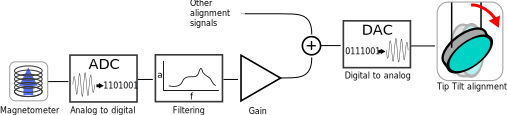
\includegraphics{figs-jitter/magffblockdiag.pdf}
  \end{center}
  \caption[Block diagram of the magnetometer feedforward system.]{Block diagram of the magnetometer feedforward system. The signal read by an analog magnetometer is digitized and filtered. The signal is then combined with other digital alignment signals, converted to analog, and applied to the Tip Tilt alignment actuators.}
  \label{fig:magffblockdiag}
\end{figure}

A magnetometer was installed and a feedforward control system was implemented in the LIGO realtime system for digital signal processing. %NL%
The feedforward system read the digitized 3-axis magnetometer signal, performed filtering, and fed the filtered signal to the Tip Tilt pitch and yaw actuators. %NL%
A diagram of the system may be seen in Figure \ref{fig:magffblockdiag}. %NL%


\begin{figure}
  \begin{center}
  \leavevmode
  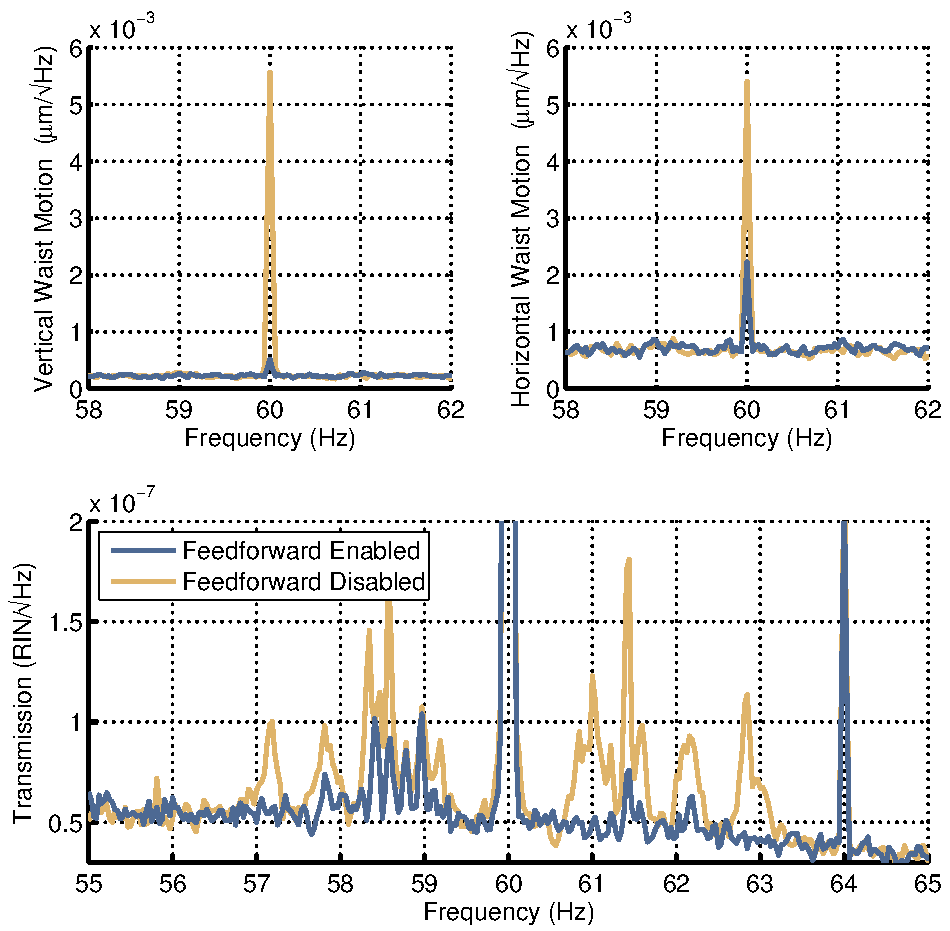
\includegraphics{figs-jitter/magffperformance.pdf}
  \end{center}
  \caption[Measurement of the performance of the magnetometer feedforward system.]{Measurement of the performance of the magnetometer feedforward system. The feedforward system was tuned to minimize the beam motion as measured by the OMC quadrant photodetectors (shown in both top panels). The beam jitter reduction leads to a reduction of the highly variable sidebands structures around the 60Hz line.}
  \label{fig:magffperformance}
\end{figure}

To reduce the 60Hz jitter peak, the signal filtering was tuned to minimize the presence of 60Hz motion measured by the OMC QPDs. %NL%
When correctly tuned, the feedforward system was able to significantly reduce the magnitude of the sidebands around 60Hz in the LIGO sensitivity spectrum. %NL%
The perfomance of the magnetometer feedforwad system is shown in Figure \ref{fig:magffperformance}.

Such a feedforward servo is beneficial whenever one has a signal which is coherent with the source of high frequency jitter noise. %NL%
Because of the bilinear coupling of beam jitter, removal of even narrow, single frequency, components of beam motion can reduce broadband sources of noise in one's data. %NL%
With only the magnetometer signal, it would not be possible to perform off-line subtraction of the sidebands around 60Hz from the final data stream. %NL%
However, it has been shown that it is possible to combine several signals, in a nonlinear way, to subtract sources of bilinear-coupled noise from off-line data \cite{G1200197,G1200288}. %NL%
This rather impressive technique has already been shown to be well suited for reduction of beam jitter noise and has truly great potential for future interferometers.

\section{The relationship of alignment control and beam jitter}
% depending on bandwidth, alignment system can remove low/DC or high. Though not if you are using a beacon system. Also beware of fringe wrapping.
As discussed in Chapter \ref{ch:beacon}, a standard cavity alignment control system is designed to minimize the \TEM{01} and \TEM{10} mode content incident on the cavity. %NL%
We have also just seen that any misalignment increases the linear coupling of beam jitter noise to the cavity transmission signal. %NL%
This connection is manifestly clear in the case of a dither alignment servo, where beam jitter is purposely induced on the beam, and the servo obtains optimum alignment by minimizing the coupling of the dither frequency in transmission. %NL%
If the DC and low frequencies of the alignment error can be sufficiently supressed by a control system, the beam jitter coupling is consequently reduced.

%Attempts were made in Enhanced LIGO to directly reduce the high frequency beam jitter on the OMC with a high bandwidth alignment servo. For sufficiently high control bandwith, it was seen that an increase in gain would cause an increase in broadband noise in the OMC transmission. One possible mechanism for the increased noise \com{OMC backscatter} \cite{T060303}.

We break this relationship between alignment optimization and jitter coupling minimization when a beacon or optimal style alignment system is used as desribed in Section \ref{sec:beaconalignment}. %NL%
Because the carrier frequency component is often the dominant contribution to the total power of the transmitted signal, it is usually the case that beam jitter noise orignating from the carrier is dominant over other frequency components. %NL%
Alignment schemes which optimize the alignment of the audio frequency signal sidebands will disregard the HOM content of the carrier beam, and thus may increase beam jitter coupling. %NL%
This additional beam jitter coupling may be mitigated by control of the relative modal content of the audio sidebands and the carrier, which will be discussed in the following section.

\section[Modification of the relative modal content of the carrier and audio sidebands]{Modification of the relative modal content of the carrier and audio sidebands\footnote{This section will satisfy as mearly a record of some lore learned during Enhanced LIGO. It is not intended to provide a quantitative model, but merely act as a guide for future efforts.}}

After the implementation of the beacon alignment system in Enhanced LIGO, some beam jitter peaks of unknown origin remained in the sensitive region of the detector. %NL%
It was discovered that the height of these peaks were controlable by modifying the beam position on the antisymmetric port alignment sensor\footnote{In Initial/Enhanced LIGO, this was known as WFS1.} of the main interferometer alignment control system. %NL%
We postulated that because of offsets in the readout of the interferometer alignment signals, changing the beam position would change the error point offsets of the alignment feedback system of the main interferometer. %NL%
The antisymmetric port signal primarily feeds back to the differential alignment mode of the ETMs. %NL%
It was thought that this lead to a redistribution of the modal content of the carrier field exiting the antisymetric port of the interferometer relative to the fields of the audio sidebands. %NL%
One could imagine that the position of a local minimum, with respect to alignment, of the carrier transmission could be moved into coincidence with the optimal alignment point of the signal fields. %NL%
Attempts were made to instead directly inject offsets into the alignment error signals to produce the same effect, but they were never as successful as varying the pointing on the alingment sensor.

\chapter{Automatic mode matching of an output mode cleaner}
\com{change degree to degrees}
In order for a laser beam to resonant in an optical cavity, it is necessary that the transverse profile of the wavefronts of the incident beam overlap with the wavefronts of the resonant mode in the cavity. %NL%
If this is not the case, subsequent round trip reflections around the cavity will not interfere constructively with the incident wave and resonance will not occur. %NL%
This is usually manifested in the incoming wavefronts having either the wrong transverse beam size, or the wrong wavefront radius of curvature. %NL%
These incongruities are commonly referred to as a mode mismatch. %NL%
In general, some component of the incident beam will overlap with the cavity mode so some resonance is possible, but the incorrectly matched components are largely reflected from the cavity. %NL%
In the case of an output mode cleaner, mode mismatch of the signal field will lead to a reduction in the final detected signal to noise ratio, much as is the case with misalignment.

\section{Mode matching in the modal picture}
As we have seen in section \ref{sec:alignmentsomething}, if a beam incident on a cavity is misaligned, the beam will have components in the n+m=1 order modes when decomposed into the modal basis of that cavity. %NL%
Another way of saying this is that the n+m=1 modes carry the alignment (or misalignment) information about the beam. %NL%
Mode matching is analogous to this situation where instead of the n+m=1 components which represent misalignment, the n+m=2 components are the ones responsible for mode mismatching.

One notable difference to alignment is that due to the Gouy phase shift being proportional to the mode order, the rotation of the mismatching mode is twice that of the alignment mode, with respect to the \TEM{00} mode.
\com{Describe how the n+m=2 modes rotate as 2*gouy phase.}

\section{Mode matching degrees of freedom}

\com{Show that beam waist shifting and beam size changing makes 20/02 modes}

\com{Try to develop some intuition about the 11 mode.}

\section{Sensing mode mismatch of the signal beam}
In order to sense mode mismatching, one needs a sensor which mixes the \TEM{00} mode with the n+m=2 order modes. %NL%
By analogy to split quandrant photodetectors used for sensing alignment, one may construct a split photodetector with a geometry that provides overlap between the \TEM{00} and n+m=2 modes. %NL%
This is often acheived using so-called bull's-eye photodetectors.\cite{Mueller:00}

\com{make a figure showing an example of the bullseye, also maybe show what the pupil matrix looks like}

\section{Mode matching actuators}

\com{Tip tilts with varying position}

\com{Deformable tiptilts}\cite{Canuel:11}

\com{Transmissive optics}\cite{Arain:10}

\section{A feedback control system for automatic mode matching of an output mode cleaner}


\appendix

\chapter{Practical calculations using matrices based on the optical vector space model}

\section{Collapsing a tensor of several indices into a 2D matrix}

\section{Define the free space propagator to have no phase rotation for the \TEM{00} carrier.}

\section{Units}

\section{Calculating signal to noise ratios}

%%% Local Variables: 
%%% mode: latex
%%% TeX-master: "main"
%%% End: 

\chapter{Additional notes}

\section{The control vector separation for alignment is the Gouy phase separation}
% also the fact that mode matching is a constraint
\label{sec:gouysep}
A servo system which is designed to control several degrees of freedom of a system simultaneously must be able to effectively sense and control each degree of freedom independently. %NL%
The degrees of freedom of the system define a phase space, and the sensors and actuators can be represented as vectors in this space. %NL%
Where the components of the vectors have amplitudes proportional to the sensitivity of the sensor, or the actuation strength of the actuator, in a given degree of freedom. %NL%
In order to effectively control one's system, care should be taken to ensure that these vectors sufficiently span the phase space. %NL%
If any direction does not have coverage, it will either be unsensed, or uncontrolled.

In the case of the alignment of a laser beam, there are four degrees of freedom. %NL%
These may be parametrized as the beam waist position and beam waist angle in the $x$ and $y$ directions.\footnote{Where $z$ is the direction of propagation.} For good alignment control of a laser beam using steering mirrors, for example into an optical cavity, a common piece of lore is that one must have a steering mirror `close' to the alignment target, and one steering mirror `far' from it. %NL%
But just what exactly sets the criteria for close and far?

Let us constrain ourselves to a single plane of beam alignment, such that we are only concerned with the waist position and angle in the $x$ direction. %NL%
It can be shown that the field of the beam can be represented as the \TEM{00} field with some small additional \TEM{01} field added when the displacements and misalignments are small \cite{Anderson1984}. %NL%
To first order in misalignment, the field can be written as
\begin{equation}
\label{eqn:shifttilt}
\vect{E}=\vect{00}+\left(\frac{\delta x}{w_0} + i \frac{\theta}{\theta_d}\right)\vect{01}
\end{equation}
where $\vect{mn}$ is the \TEM{mn} eigenmode, $\delta x$ is the beam position displacement, $w_0$ is the beam waist radius, $\theta$ is the beam tilt angle, and $\theta_d=\lambda/(\pi w_0)$ is the divergence angle. %NL%
Therefore we may frame the problem of controlling the beam position and angle by our ability to control the real and imaginary quadratures of the amplitude of the \TEM{01} component. %NL%
Thus a `good' alignment system will be one in which the ability of the system to actuate on the real and imaginary quadratures of the \TEM{01} field is well separated.

We will represent our alignment system as two steering mirrors labeled A and B. %NL%
The beam first reflects from mirror A, travels some distance, then reflects from mirror B. %NL%
We will consider a vector space of the \TEM{00} and \TEM{01} modes as basis vectors. %NL%
From Equation \ref{eqn:mirrortilt} we see that, in this representation, the operator for mirror A is
\begin{equation}
%\oper{M}_{\rm A}=\oper{I}-2i\Theta_{\rm A}\left(\vect{00}\form{01}+\vect{01}\form{00}\right),
\oper{M}_{\rm A} \doteq \ms 1 &-2i\Theta_{\rm A}\\-2i\Theta_{\rm A} & 1\me
\end{equation}
where $\Theta_{\rm A}$ is the alignment angle of mirror A. %NL%
A similar expression holds for mirror B.

Between mirrors A and B, we allow the laser to propagate some distance. %NL%
Along with the propagation phase which is common to all modes, the \TEM{01} mode experiences the additional Gouy phase $\eta$. %NL%
The propagation operator is
\begin{equation}
%\oper{P}=e^{i\phi}\left(\vect{00}\form{00}+e^{i\eta}\vect{01}\form{01}\right),
\oper{P}\doteq e^{i\phi}\ms 1&0\\0&e^{i\eta}\me
\end{equation}
where $\phi$ is the overall phase common to all modes.

To first order in angles and ignoring the overall phase, the operator of the entire alignment system is
\begin{equation}
\oper{M}_{\rm B}\oper{P}\oper{M}_{\rm A}\doteq
\ms 1 & -2i\left(\Theta_{\rm A}+e^{i\eta}\Theta_{\rm B}\right)\\
-2i\left(e^{i\eta}\Theta_{\rm A}+\Theta_{\rm B}\right) & e^{i\eta} \me.
\end{equation}
If we apply this to a pure \TEM{00} field on the input, the output field is
\begin{equation}
\vect{E}_{\rm{out}}=\vect{00}-2i\left(e^{i\eta}\Theta_{\rm A}+\Theta_{\rm B}\right)\vect{01}.
\end{equation}
Comparing this to Equation \ref{eqn:shifttilt}, we see that mirror B actuates exclusively on the beam angle, while for mirror A, the amount of position or angle actuation depends on the Gouy phase propagation between the two mirrors, $\eta$. %NL%
If $\eta=\pi/2$, then mirror A only actuates on position and the two actuators are completely separated in actuator phase space. %NL%
In fact, the angle between the actuators in phase space is just $\eta$.

Intuitively, this may be understood by the fact that the \TEM{01} mode has an extra rotation relative to the \TEM{00} mode, this is the Gouy phase. %NL%
Once one of the mirrors has actuated on the beam, we must let the quadrature that was actuated on rotate away so that we may actuate on the perpendicular quadrature. %NL%
This rotation is what causes angles in the near field to rotate into positions in the far field. %NL%


The treatment of sensing is quite similar, in that case, it is the demodulation operator (Equation \ref{eqn:spacedemod}) which connects the \TEM{00} and \TEM{01} modes, and again, the Gouy phase dictates the sensor separation.

As a final thought, if one were designing an actuation system for modes of higher order than \TEM{01}, the propagation operator matrix element for a \TEM{mn} mode would be $e^{(m+n)\eta}$. %NL%
This would cause the optimal control separation (a phase space angle of $\pi/2$) to occur at $\eta=\frac{1}{m+n}\frac{\pi}{2}$. %NL%
Thus, mode matching sensors and actuators, which operate on $m+n=2$ modes, must have  $\eta=\pi/4$ separation for optimal performance.

\section{Dither sensing is a measurement of a partial derivative}
\label{sec:dithersens}
Suppose one has a sensor which measures some physical quantity $P$, which depends on a variable $\theta$ which is controlable by some means of actuation. %NL%
A modulation is injected into the variable $\theta$ such that
\begin{equation}
\theta = \theta_0+\alpha \sin[\omega t],
\end{equation}
where $\alpha \ll 1$ is the modulation depth, and $\omega$ is the modulation frequency. %NL%
The resulting behavior of $P$ is
\begin{equation}
P(\theta)=P(\theta_0+\alpha \sin[\omega t])\approx P(\theta_0)+\frac{\partial P}{\partial \theta}(\theta_0)\alpha \sin[\omega t] + \ldots
\end{equation}
Thus the amplitude of the $\omega$ frequency component, which can be determined by demodulation, is proportional to the partial derivative of the measured quantity with respect to the controlled variable. %NL%
This is the basic mechanism behind dither sensing.
\section{Conventions for the coefficient of amplitude transmission and reflectivity of beamsplitters}
Imagine a beam with complex electric field amplitude $E_0$ striking a partially reflective boundary. %NL%
The beam will be split into two resultant beams, a transmitted beam and reflected. %NL%
Define the transmitted beam as a complex coefficient, $t$, multiplied by the incident beam. %NL%
Similarly, the reflected beam will be multiplied by $r$. %NL%
This is shown in Figure \ref{fig:mrfig1}. %NL%
Note: we make no assumption about the value of these coefficients. %NL%
At all times we will ignore phase shifts due simply to propagation, so the $ik\delta z$ phase is always divided out.

\begin{figure}
  \begin{center}
  \leavevmode
  \subfloat[The incident beam.]{\label{fig:mrfig1}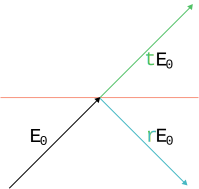
\includegraphics{figs-ap-notes/mrfig1.pdf}}
  ~
  \subfloat[The time reversed situation.]{\label{fig:mrfig2}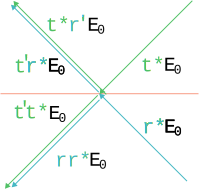
\includegraphics{figs-ap-notes/mrfig2.pdf}}
  \end{center}
  \caption{Diagram of the interaction of a beam with a beamsplitter.}
  \label{fig:mrfig}
\end{figure}

Imagine the time reversed process of the two resultant beams. %NL%
In the phasor space of the electric field, time reversal requires the complex conjugation operation. %NL%
The blue beam will be split into two beams for which we will use the same coefficients of transmission and reflection as in the case already considered, because it interacts with the boundary from the same direction. %NL%
However, we will assume that the green beam, which is hitting the boundary from the other side, has different coefficients, $t'$ and $r'$. %NL%
This situation is shown in Figure \ref{fig:mrfig2}.

Now, we make the assumption that this process obeys the principal of time reversal symmetry.\footnote{This also implicitly assumes there are no losses.} Thus the result of the second case should match the initial conditions of the first case. %NL%
The the two beams above the boundary should interfere destructively, while the two below should reproduce the original input beam. %NL%
This gives us two equations.
\begin{align*}
rr^*+t't^*&=1,\\
t'r^*+r't^*&=0.
\end{align*}
Solving for $t$ gives
\begin{equation}
t=-ie^{i\phi/2}\sqrt{1-|r|^2},
\end{equation}
where $e^{i\phi}\equiv r'/r^*$. %NL%
The two most common conventions choose $r$ to be real and $\phi$ to either be $\pi$, leading to the $r=-r'$ with $t$ real convention, or $2\pi$, leading to the $r=r'$ with $t=i\tau$ for $\tau$ real convention.

\section{The focusing power of a displaced mirror}
When optimizing the mode matching of a laser beam into an optical cavity, there are typically two ways to modify the focusing of the beam. %NL%
One is to change the optical elements for others with a differing focal length, or in some extreme cases, by using optical elements with a variable focusing power (Chapter \ref{ch:modematching}). %NL%
The second method is to modify the position of the optical elements, this changes the free propagation distance between the elements, and hence, the locations and sizes of the focused beams.

The question to be addressed is ``How does one compare a change in focal length to a change in position of the optic in a quantitatively equivalent way?'' %NL%
For small perturbations of mode matching, a change in the focus of a beam can be considered as coupling between the \TEM{00} mode with the second order ($m+n=2$) modes of the beam \cite{Anderson1984}. %NL%
For a variable focusing power, this is given in Equation \ref{eq:matrixelement}. %NL%
Here we aim to calculate a similar expression for a mirror \com{and a lens?} that has been displaced along the optic axis.

\com{TBD}
\section{The second order HOMs}
\com{What do the \TEM{02} 20 and 11 modes look like?}


\begin{figure}
  \begin{center}
  \leavevmode
  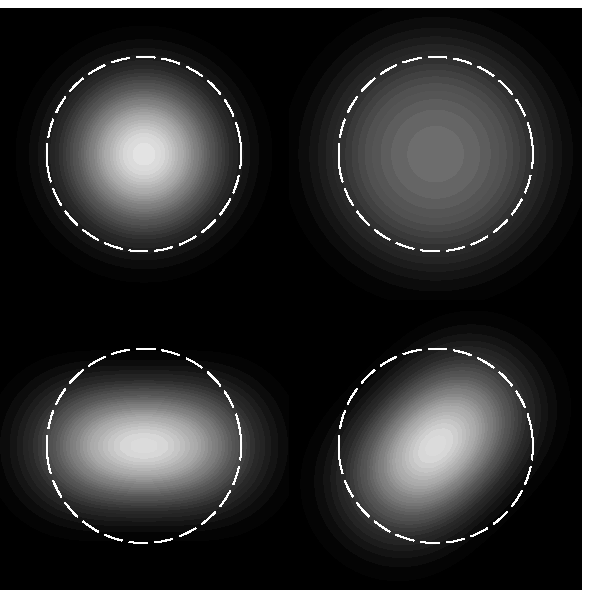
\includegraphics{figs-ap-notes/secondordermodes.pdf}
  \end{center}
  \caption[ADD ME]{ADD ME}
  \label{fig:secondordermodes}
\end{figure}
\chapter{Common misconceptions about laser interferometer gravitational-wave antenn\ae}

\section{Why LIGO has two arms}

\section{The sensitivity/bandwidth ``tradeoff''}

%%% Local Variables: 
%%% mode: latex
%%% TeX-master: "main"
%%% End: 



%% This defines the bibliography file (main.bib) and the bibliography style.
%% If you want to create a bibliography file by hand, change the contents of
%% this file to a `thebibliography' environment.  For more information 
%% see section 4.3 of the LaTeX manual.
\begin{singlespace}
\bibliography{mainb}
\bibliographystyle{unsrtnat}
\end{singlespace}


\end{document}

